% !TeX program = LuaLaTeX--shell-escape

\documentclass[b5paper,11pt,openany]{guidatematica}
\ProvidesFile{guidalua.tex}[2021/03/28 v0.4 Guida al linguaggio Lua per LuaTeX]
\GetFileInfo{guidalua.tex}
\setmonofont[Scale=0.82]{Fira Mono}
\usepackage{sourcecode}

\fvset{fontsize=\small}
\usepackage[
    colorlinks=true,
    linkcolor=blue,
    citecolor = blue,
    urlcolor = blue,
    pdftitle={Guida al linguaggio Lua per LuaTeX},
    pdfauthor={Roberto Giacomelli},
    pdfsubject={Guida tematica del GuIT},
    pdfkeywords={Lua, LuaTeX, guida, programming}
]{hyperref}
\usepackage{exercise}
\renewcounter{Exercise}[chapter]
\renewcommand{\ExerciseHeader}{\noindent\textsc{esercizio \ExerciseHeaderNB}}

\usepackage{tcolorbox}
\tcbuselibrary{skins}
\tcbset{
    sharp corners=all,
    colback=verdeguit!10!white,
    colframe=verdeguit!35!white,
    bicolor,
    colbacklower=white,
    boxrule=0.3pt,
    leftrule=2pt,
    fonttitle=\bfseries,
    fontupper=\small,
    fontlower=\small
}
\tcbuselibrary{documentation}
\tcbset{doc marginnote={
    colframe=verdeguit,
    colback=verdeguit!5!white,
    width=21mm,
    enlarge left by=-7mm
    }
}

\usepackage{siunitx}
\sisetup{output-decimal-marker=\virgoladecimale}

\frenchspacing

\newcommand\tcmd[1]{\normalfont\texttt{#1}}
\newcommand\key[1]{\normalfont\texttt{#1}}
\newcommand\code[1]{\normalfont\texttt{#1}}
\newcommand\fn[1]{\normalfont\texttt{#1()}}

\begin{document}
\author{Roberto Giacomelli}
\date{\filedate{} --- \fileversion}
\title{Guida al linguaggio Lua per \LuaTeX}
\subtitle{
\begin{tikzpicture}[scale=0.82]
\node at (-2.31-0.72, 0) {};
\draw[fill,verdeguit] (0,0) circle (2.2);
\draw[fill,verdeguit] (2.31, 2.31) circle (0.72);
\draw[fill, white] (0.8,0.8) circle (0.72);
\end{tikzpicture}
\vspace*{8.5ex}
}
\maketitle

\tableofcontents
\newpage


% presentazione della guida e informazioni di base per eseguire gli esempi

\chapter{Presentazione}

\section{Motivazione}

Questa guida tematica è dedicata alla programmazione in Lua all'interno dei
motori di composizione del sistema \TeX.

Con Lua è possibile compiere sia elaborazioni generiche come l'interrogazione di
basi di dati che elaborazioni tipografiche interagendo con il compositore
interno. Con Lua rispetto a \TeX, è più semplice ed efficiente effettuare
calcoli numerici o avvalersi di avanzate librerie esterne.

La nuova generazione di compositori amplia così notevolmente gli scenari
applicativi. Se da un lato è auspicabile che queste potenzialità diventino
disponibili per gli utenti finali per mezzo di moduli e pacchetti, dall'altro è
utile fornire dettagli ed esempi per implementare proprie soluzioni o per poter
scrivere nuovi moduli condividendone lo sviluppo con la community.

Sono certamente molte le cose da conoscere: un nuovo linguaggio molto diverso da
\TeX{}, numerosi dettagli sul funzionamento interno dei compositori Lua-powered,
nuovi problemi di organizzazione del codice, di bilanciamento tra Lua e \TeX,
eccetera. Per questo, ho pensato di contribuire con questa guida cercando di
presentare il quadro della crescente complessità del sistema.


\section{Piano della guida}

La guida è divisa in tre parti: la prima offre una panoramica rapida in forma di
\emph{tutorial} per iniziare subito con Lua seguendo i passi di un ipotetico
utente alle prese con problemi compositivi (parte \ref{partTutorial}), la
seconda tratta delle basi del linguaggio Lua (parte \ref{partFoundation}) e
contiene numerosi esercizi, e infine la terza illustra esempi applicativi con
l'uso delle librerie di composizione cn i nodi (parte \ref{partApp}).

Tra gli argomenti ci sono:
\begin{compactitemize}
\item differenza tra motore e formato di composizione \( \to \) capitolo
\ref{iichExplain},
\item basi del linguaggio Lua \( \to \) dal capitolo \ref{chAssignment},
\item tecniche di programmazione e di rappresentazione dei dati \( \to \) dal
capitolo \ref{iichRegistro},
\item la tecnologia dei nodi in Lua \( \to \) capitolo \ref{iichTartaglia}.
\end{compactitemize}


\section{Origine della guida}

Per illustrare i concetti del linguaggio ho preso spunto da un breve corso su
Lua che scrissi qualche tempo fa per il blog
\href{http://parliamodi-ubuntu.blogspot.it}{Lubit Linux} di Luigi Iannoccaro
che mi propose di realizzare un progetto di divulgazione su Lua. Luigi ha
acconsentito all'utilizzo di quegli appunti per produrre questa guida tematica.


\section{Contribuire e collaborare}

Spero che i lettori vorranno contribuire al testo inviando proprie soluzioni o
nuovi contributi piccoli o grandi. Lo si può fare attraverso lo strumento che
preferite, scrivendomi un messaggio di posta elettronica all'indirizzo
\href{mailto:giaconet.mailbox@gmail.com}{\texttt{giaconet.mailbox@gmail.com}},
oppure utilizzando il
\href{https://github.com/GuITeX/guidalua}{\texttt{repository git}} dei sorgenti
della guida, eseguendo un Pull Request o aprendo una discussione premendo il
pulsante Issues.


\section{Altre risorse}

La risorsa principale per imparare Lua, a cui si rimanda per tutti gli
approfondimenti, è certamente il PIL \cite{PIL} acronimo del titolo del libro
\emph{Programming In Lua} di Roberto Ierusalimschy, principale Autore di Lua.
Questo testo non solo è completo e autorevole ma è anche ben scritto e
composto\footnote{Tra l'altro il libro ufficiale su Lua viene composto in
\LaTeX{} e commercializzato per contribuire allo sviluppo del linguaggio
stesso.}.

La seconda importante risorsa su Lua si trova in rete all'indirizzo
\href{https://www.lua.org/manual/5.3/}{\texttt{www.lua.org/manual/5.3/}} ed è il
\emph{reference} del linguaggio \cite{web:luaref} con le specifiche di sintassi,
metametodi, funzioni di libreria, C API eccetera.

Quanto a \LuaTeX{} il riferimento è il suo manuale \cite{prg:luatex} che, come
quasi tutta la documentazione nel sistema \TeX{}, può essere visualizzato a
video con il comando da terminale:
\begin{Verbatim}[numbers=none]
$ texdoc luatex
\end{Verbatim}


\section{Note di lettura}

Nei listati compilabili riportati nella guida compare alla prima linea la
\emph{riga magica}, un commento utile per dare istruzioni all'editor sul
compilatore da usare, ma che qui informerà il lettore per aiutarlo a stabilire
il contesto del codice.

Se presente nel progetto, alla seconda riga dei listati si troverà invece il
nome del file che il lettore potrà scaricare ed eseguire per i propri
esperimenti dal \href{https://github.com/GuITeX/guidalua}{\texttt{repository
git}}.

Nella parte \ref{partFoundation} ho cercato di non dare per scontati i concetti
fondamentali della programmazione. Ovviamente il lettore già preparato procederà
più velocemente nel prendere dimestichezza con Lua. Ho invece escluso dalla
guida \TeX{}, per esempio non spiegando come si definisce una macro utente o
come si lavora con il formato \LaTeX3. Rimando senza indugio alla copiosa
documentazione disponibile a cominciare da quella scaricabile dal sito \GuIT.

Diamo quindi inizio a questa nuova avventura lunare.

% end of file


\mainmatter*

\part{Tutorial}
\label{partTutorial}


% esercitazioni semplici con richiami ai fondamenti


\chapter{Let's start with Lua}
\label{chGo}

Per dare l'idea di come si possa usare Lua all'interno del sistema di
composizione \TeX{}, questa prima parte della guida è in forma di
\emph{tutorial} cioé di brevi resoconti dei progressi compiuti da un ipotetico
utente \LuaLaTeX{} indaffarato nel risolvere alcuni problemi con i suoi
documenti: fare calcoli con una calcolatrice o comporre una tabella ripetitiva.

Nel margine di pagina il lettore troverà i rimandi di approfondimento. I
tutorial infatti non hanno l'obiettivo di spiegare la programmazione Lua ma di
introdurne l'utilità.


\section{La calcolatrice}

Una calcolatrice, una macro \cs{expr} che accetti un'espressione numerica e
ne stampi il risultato. Sarebbe davvero utile non dover più calcolare a
parte il risultato e riportarlo nel sorgente del documento \LaTeX{} con un copia
incolla o peggio a mano.

Tentiamo qualcosa di molto semplice con Lua, assegnare l'espressione a una
variabile per poi stamparla nel documento:
%
\tcbdocmarginnote[enlarge top initially by=\margindown]{%
Lua in \TeX\\
\gotosec{} \ref{secLuaInLuaLaTeX}}
%
\tcbdocmarginnote[enlarge top initially by=\dimexpr\margindown+9mm\relax]{%
Variabili locali\\
\gotosec{} \ref{secGlobaleLocale}, \gotosec{} \ref{secFondLocaleGlobale}}
%
\tcbdocmarginnote[enlarge top initially by=\dimexpr\margindown+18mm\relax]{%
\fn{tex.print}\\
\gotosec{} \ref{secPassaggioDati}}
%
\begin{Verbatim}
% !TeX program = LuaLaTeX
% filename: app-start/E0-001-expr.tex
\documentclass{article}
\newcommand\expr[1]{\directlua{
    local result = #1
    tex.print(tostring(result))
}}
\begin{document}
Finalmente una calcolatrice:
\( 1.24 (7.45 + 11.21) = \expr{1.24*(7.45 + 11.21)}\)
\end{document}
\end{Verbatim}

\newcommand\expr[1]{\directlua{
    local result = #1
    tex.print(tostring(result))
}}
compilando con \LuaLaTeX{} il risultato è:
\begin{tcolorbox}
Finalmente una calcolatrice: \( 1.24 (7.45 + 11.21) = \expr{1.24*(7.45 + 11.21)}\)
\end{tcolorbox}

Un buon inizio. Nel sorgente all'interno della macro \cs{directlua} il primo
argomento è stato sostituito con l'espressione che viene poi valutata da Lua.
Nessun pacchetto aggiuntivo caricato, qualsiasi espressione numerica è lecita, e
questo solo e soltanto usando Lua incluso in \LuaTeX.

Funziona anche con le stringhe, a patto di delimitarne il valore, e con le
espressioni booleane. Proviamo:
\begin{tcolorbox}
\verb=\( 56.9 > 78.42 \) è \texttt{\expr{ 56.9 > 78.42 }}=
\tcblower
\( 56.9 > 78.42 \) è \texttt{\expr{ 56.9 > 78.42 }}
\end{tcolorbox}

E se si volessero sostituire le rappresentazioni testuali dei valori vero e
falso? Ecco la modifica:
%
\tcbdocmarginnote[enlarge top initially by=\margindown]{%
Ciclo \key{if}\\
\gotosec{} \ref{secFondCicloIf}}
%
\tcbdocmarginnote[enlarge top initially by=\dimexpr\margindown+9mm\relax]{%
Tipo \key{boolean}\\
\gotosec{} \ref{secFondManciataTipi}}
%
\tcbdocmarginnote[enlarge top initially by=\dimexpr\margindown+18mm\relax]{%
Operatore ternario\\
\gotosec{} \ref{secFondOperatoreTernario}}
%
\begin{Verbatim}
\newcommand\expr[1]{\directlua{
    local result = #1
    if type(result) == "boolean" then
        result = result and "vero" or "falso"
    end
    tex.print(tostring(result))
}}
\end{Verbatim}

\renewcommand\expr[1]{\directlua{
    local result = #1
    if type(result) == 'boolean' then
        result = result and 'vero' or 'falso'
    end
    tex.print(tostring(result))
}}

Un semplice test ci conforterà sulla correttezza del codice:
\begin{tcolorbox}[sidebyside]
\begin{Verbatim}[numbers=none, xleftmargin=0pt]
\expr{100 == 100 and 7 > 3}
\expr{-10 < -100}
\end{Verbatim}
\tcblower
\expr{100 == 100 and 7 > 3}\\
\expr{-10 < -100}
\end{tcolorbox}

Si, funziona ma andiamo avanti. Vorrei poter regolare l'arrotondamento del
risultato numerico della calcolatrice ricorrendo a un argomento opzionale
separato dall'espressione da una virgola:
%
\tcbdocmarginnote[enlarge top initially by=\margindown]{%
\fn{string.format}\\
\gotosec{} \ref{secFondStringFormat}}
%
\begin{Verbatim}
\newcommand\expr[1]{\directlua{
    local result, dec = #1
    if type(result) == "boolean" then
        result = result and "vero" or "falso"
    elseif type(result) == "number" and dec then
        local perc = string.char(37)
        local fmt1 = perc..perc.."0."..perc.."df"
        local fmt2 = string.format(fmt1, dec)
        result = string.format(fmt2, result)
    end
    tex.print(tostring(result))
}}
\end{Verbatim}

\renewcommand\expr[1]{\directlua{
    local result, dec = #1
    if type(result) == 'boolean' then
        result = result and 'vero' or 'falso'
    elseif type(result) == 'number' and dec then
        local perc = string.char(37)
        local fmt1 = perc..perc..'0.'..perc..'df'
        local fmt2 = string.format(fmt1, dec)
        result = string.format(fmt2, result)
    end
    tex.print(tostring(result))
}}

Stavolta il codice perde un po' di chiarezza perché non è possibile usare
direttamente il carattere percento \code{\%} che verrebbe interpretato come
inizio di un commento nel costruire le stringhe di formato. Ovviamente questo
non succederebbe se il codice fosse in un file separato o se fosse racchiuso in
un ambiente \pack{luacode} dell'omonimo pacchetto \LaTeX.

Mettiamo alla prova la modifica alla macro \cs{expr}:
\begin{tcolorbox}
\verb|\(\sqrt{2} + \sqrt{3} \approx \expr{ 2^0.5 + 3^0.5, 2}\)|
\tcblower
\(\sqrt{2} + \sqrt{3} \approx \expr{ 2^0.5 + 3^0.5, 2}\)
\end{tcolorbox}

Potremo trovare una sintassi un po' più chiara, tuttavia occupiamoci di un
problema più urgente: poter usare funzioni matematiche come seno e coseno. Se
scrivessimo \verb=\expr{sin(1)^2 + cos(1)^2}= non otterremo il valore unitario
ma un errore. Dovremo infatti usare la scomoda notazione
\code{math.}\meta{funzione}/\meta{costante} come in
\verb=\expr{math.cos(math.pi)}= invece della più naturale \verb=\expr{cos(pi)}=.
Ma ci vuole poco a riassegnare le funzioni a nomi locali per far si che
l'identità trigonometrica precedente sia un'espressione valida:
\begin{Verbatim}
\newcommand\expr[1]{\directlua{
    local cos = math.cos
    local sin = math.sin
    local result, dec = #1
    if type(result) == "boolean" then
        result = result and "vero" or "falso"
    elseif type(result) == "number" and dec then
        local perc = string.char(37)
        local fmt1 = perc..perc.."0."..perc.."df"
        local fmt2 = string.format(fmt1, dec)
        result = string.format(fmt2, result)
    end
    tex.print(tostring(result))
}}
\end{Verbatim}

\renewcommand\expr[1]{\directlua{
    local cos = math.cos
    local sin = math.sin
    local result, dec = #1
    if type(result) == 'boolean' then
        result = result and 'vero' or 'falso'
    elseif type(result) == 'number' and dec then
        local perc = string.char(37)
        local fmt1 = perc..perc..'0.'..perc..'df'
        local fmt2 = string.format(fmt1, dec)
        result = string.format(fmt2, result)
    end
    tex.print(tostring(result))
}}

Una prova della calcolatrice potenziata con le funzioni trigonometriche ci dirà
se tutto funziona ancora bene:
\begin{tcolorbox}
\begin{Verbatim}[numbers=none,xleftmargin=0pt]
\(\sin^2(1/2) + \cos^2(1/2) = \expr{sin(0.5)^2 + cos(0.5)^2, 8}\).
\end{Verbatim}
\tcblower
\(\sin^2(1/2) + \cos^2(1/2) = \expr{sin(0.5)^2 + cos(0.5)^2, 8}\).
\end{tcolorbox}
e per un'espressione booleana:
\begin{tcolorbox}
\begin{Verbatim}[numbers=none,xleftmargin=0pt]
A \( 1/3 \) l'identità è \emph{\expr{sin(1/3)^2 + cos(1/3)^2 == 1}}
\end{Verbatim}
\tcblower
A \( 1/3 \) l'identità è \emph{\expr{sin(1/3)^2 + cos(1/3)^2 == 1}}
\end{tcolorbox}

Finora ogni nuova funzionalità aggiunta alla calcolatrice non ha presentato
difficoltà. Possiamo inserire o meno il risultato in ambiente matematico,
arrotondarlo al numero di decimali desiderato e usare funzioni matematiche
dell'efficiente libreria in virgola mobile di Lua, un linguaggio che si sta
dimostrando semplice da usare e molto efficace.

Continuamo con un nuovo passo: aggiungere costanti numeriche definite
dall'utente, una sorta di \emph{funzione di memoria} della calcolatrice. Per
inserire variabili letterali in un'espressione abbiamo bisogno che il loro
valore numerico sia inizializzato ma non possiamo ricorrere alla stessa tecnica
con cui abbiamo risolto l'inserimento delle funzioni trigonometriche.

Non è possibile infatti codificare variabili locali senza conoscerne il nome,
perché è un dato fornito dall'utente. Servirebbe una sorta di metaprogrammazione
come con le macro dei linguaggi compilati. Leggendo più a fondo la
documentazione di Lua, si scopre che è possibile intervenire sull'ambiente delle
variabili globali \code{\_ENV}\footnote{Per ulteriori informazioni
sull'\emph{environment} di Lua rimando al PIL dove si trova un intero capitolo
ad esso dedicato.} di un \emph{chunk}, e anzi, a ben vedere il problema di
rendere visibili simboli di costanti è lo stesso che quello di rendere
disponibili nell'espressione le funzioni matematiche con nomi abbreviati.
Facciamo un tentativo ripartendo con il codice da zero:

\tcbdocmarginnote[enlarge top initially by=\margindown]{%
Tipo \code{table}\\
\gotosec{} \ref{iChTabella}}
%
\tcbdocmarginnote[enlarge top initially by=\dimexpr\margindown+9mm\relax]{%
Iteratore \fn{pairs}\\
\gotosec{} \ref{secFondPairsIterator}}
%
\begin{Verbatim}
\directlua{
calclib = {}
for name, object in pairs(math) do
    calclib[name] = object
end
}
\newcommand\expr[1]{\directlua{
do
    local _ENV = calclib
    ans = #1
end
tex.print(tostring(calclib.ans))
}}
\end{Verbatim}

Stiamo sfruttando una tecnica piuttosto interessante: all'interno di un blocco
viene riassegnata localmente la variabile \code{\_ENV} a \code{calclib}, una
tabella in cui vi abbiamo riversato tutte le funzioni e le costanti matematiche
della libreria \code{math} di Lua. Alla riga 10, tutti quei nomi saranno
visibili come variabili globali proprio quando l'espressione deve essere
valutata.

Non solo, come effetto collaterale, il risultato dell'ultimo calcolo sarà
disponibile nella successiva espressione memorizzato nella variabile \code{ans}
come succede con altri tool matematici! Proviamolo:
%
\directlua{
calclib = {}
for name, object in pairs(math) do
    calclib[name] = object
end
}
\renewcommand\expr[1]{\directlua{
do
    local _ENV = calclib
    ans = #1
end
tex.print(tostring(calclib.ans))
}}
%
\begin{tcolorbox}[sidebyside]
\begin{Verbatim}
\expr{pi/4}\\
\expr{cos(ans)}\\
\expr{acos(ans)}
\end{Verbatim}
\tcblower
\expr{pi/4}\\
\expr{cos(ans)}\\
\expr{acos(ans)}
\end{tcolorbox}

Molto bene. Non ci resta che aggiungere con la stessa tecnica la memorizzazione
delle costanti attivando l'argomento opzionale della macro \cs{expr}. Tra le
parentesi quadre potremo fornire all'espressione una lista di costanti nel
formato chiave/valore con separatore il carattere virgola.

Memorizzeremo le costanti indicate dall'utente solamente se il loro nome non è
già stato utilizzato o se non è un un nome di funzione. Inoltre, specificando
una stringa solo come chiave tra le opzioni, potremo implementare la
memorizzazione del risultato dell'espressione stessa, così che sia poi
riutilizzabile:
\begin{Verbatim}
\directlua{
calclib = {}
for name, object in pairs(math) do
    calclib[name] = object
end
}
\newcommand\expr[2][]{\directlua{
do
    local error, pairs, assert, type = error, pairs, assert, type
    local _ENV = calclib
    local opt = {#1}
    local mem = opt[1]; opt[1] = nil
    for c, val in pairs(opt) do
        if _ENV[c] then
            error("Duplicated key '"..c.."' in constant name")
        else
            _ENV[c] = val
        end
    end
    ans = #2
    if mem then
        assert(type(mem) == "string")
        if _ENV[mem] then
            error("Duplicated key '"..mem.."' in memory index")
        else
            _ENV[mem] = ans
        end
    end
end
tex.print(tostring(calclib.ans))
}}
\end{Verbatim}

\renewcommand\expr[2][]{\directlua{
do
    local error, pairs, assert, type = error, pairs, assert, type
    local _ENV = calclib
    local opt = {#1}
    local mem = opt[1]; opt[1] = nil
    for c, val in pairs(opt) do
        if _ENV[c] then
            error([[Duplicated key ']]..c..[[' in constant name]])
        else
            _ENV[c] = val
        end
    end
    ans = #2
    if mem then
        assert(type(mem) == [[string]])
        if _ENV[mem] then
            error([[Duplicated key ']]..mem..[[' in memory index]])
        else
            _ENV[mem] = ans
        end
    end
end
tex.print(tostring(calclib.ans))
}}

Eccone un esempio:
\begin{tcolorbox}
\begin{Verbatim}[numbers=none,xleftmargin=0pt]
\( b = \expr[b=10, h=20]{b} \), % oppure \expr["b", h=20]{10}
\( h = \expr{h} \),
\( M = \expr[m = 1000]{m}\), % oppure \expr["m"]{1000}
\( \sigma = M/W_\mathrm{x} = \expr[w=(b*h^2)/6]{m/w}\).
\end{Verbatim}
\tcblower
\( b = \expr[b = 10]{b} \),
\( h = \expr[h = 20]{h} \),
\( M = \expr[m = 1000]{m}\),
\( \sigma = M/W_\mathrm{x} = \expr[w=(b*h^2)/6]{m/w}\).
\end{tcolorbox}

Poiché anche i valori assegnati alle costanti sono valutati da Lua \emph{dopo}
la modifica dell'environment, anche per le costanti nelle opzioni della macro
\cs{expr} è possibile assegnare espressioni usando tutte le funzioni matematiche
e tutte le costanti precedentemente definite. Da questo punto in poi, possiamo
presentare il valore di \( W_\mathrm{x} \) scrivendo nel sorgente
\verb=\expr{w}= che da \expr{w}.

\subsection{Conclusioni}

Tutte le principali funzionalità della calcolatrice sono state implementate in
Lua, certo non tutte. Per esempio potremo far eseguire calcoli coinvolgendo
anche registri contatori o dimensionali di \TeX{}, per esempio per fornire
coordinate in un disegno, oppure considerare che constanti dai nomi speciali
come \code{M1}, \code{M2} eccetera si comportino come registri di memoria della
calcolatrice e quindi che possano essere sovrascritti o possano funzionare da
accumulatori.

% end of file




\section{Tabella dei pesi}

Dopo la calcolatrice si presenta un'altro problema compositivo: una tabella che
riporta per vari diametri, area e peso della barra d'acciaio di lunghezza di un
metro. I diametri variano da 6 a 32 millimetri con passo di 2 per i soli numeri
pari. 

L'idea è definire una sorta di iteratore che generi i valori delle righe della
tabella una dopo l'altra. Per esempio, se volessimo una tabella con due colonne,
la prima con gli interi da 1 a 10 e la seconda con i rispettivi quadrati,
dovremo poter scrivere solamente la funzione di calcolo e il valore finale del
contatore.

La funzione potrà essere qualsiasi purché sia definita per accettare due
argomenti: il primo è il contatore e il secondo è l'array di riga. Nel nostro
caso essa dovrà memorizzare il contatore in posizione 1 e il quadrato in
posizione 2 dell'array:
\begin{Verbatim}
local function regola(counter, r)
    r[1] = counter
    r[2] = counter^2
end
local row = Row:new(regola, 10)
\end{Verbatim}

Prima di passare al codice dell'oggetto \code{Row} verifichiamo la costruzione
della tabella in \LuaLaTeX{} notando che il metodo \fn{new} accetta proprio una
funzione come primo argomento e il valore finale del contatore come secondo
argomento: in Lua le funzioni sono valori come tutti gli altri.

L'idea originale è quindi realizzata se attribuiamo alla funzione che calcola la
generica riga della tabella il ruolo di \emph{regola} di definizione dell'intera
tabella. A ben vedere potremo fare a meno del secondo parametro per restituire
direttamente l'array di riga, tuttavia in questo modo il codice risulta più
efficiente.

\directlua{
Row = {}
Row.__index = Row
function Row:new(fn_next, start, stop, step)
    if not stop then
        start, stop = 1, start
    end
    local o = {
        fn_next = fn_next,
        start = start,
        stop = stop,
        step = step or 1
    }
    setmetatable(o, self)
    return o
end

function Row:next()
    local var = self.var
    if not var then
        var = self.start
    else
        var = var + self.step
    end
    if var <= self.stop then
        self.var = var
        local fn = self.fn_next
        fn(var, self)
        return true
    end
end
}

Il corpo del documento di prova che trovate per intero nel file indicato al
solito nella seconda riga, è il seguente:
\begin{tcolorbox}[sidebyside,righthand width=21mm]
\begin{Verbatim}
% !TeX program = LuaLaTeX
% filename: app-start/E0-003-tab.tex
\documentclass{article}
% preambolo non riportato
\begin{document}
\begin{tabular}{rr}
\directlua{
local row = Row:new(
    function (c, r) r[1] = c; r[2] = c^2 end, 10
)
local bs = string.char(92)
while row:next() do
    tex.print(row[1].."&"..row[2]..bs..bs)
end
}
\end{tabular}
\end{document}
\end{Verbatim}
\tcblower
\begin{tabular}{rr}
\directlua{
local row = Row:new(function (c, r) r[1]=c; r[2] = c^2 end, 10)
local bs = string.char(92)
while row:next() do
tex.print(row[1]..[[&]]..row[2]..bs..bs)
end
}
\end{tabular}
\end{tcolorbox}

L'implementazione della classe \code{Row} consiste in poche di linee di codice:
\begin{Verbatim}
Row = {}; Row.__index = Row
function Row:new(fn_next, start, stop, step)
    if not stop then
        start, stop = 1, start
    end
    local o = {
        fn_next = fn_next,
        start = start,
        stop = stop,
        step = step or 1
    }
    setmetatable(o, self)
    return o
end
function Row:next()
    local var = self.var
    if not var then
        var = self.start
    else
        var = var + self.step
    end
    if var <= self.stop then
        self.var = var
        local fn = self.fn_next
        fn(var, self)
        return true
    end
end
\end{Verbatim}

Possiamo considerarla come un generatore di righe. Tramite la regola
rappresentata dalla funzione e tramite i tre parametri di iterazione, ogni tipo
di dati potrà essere rappresentato in una forma tabellare. Per esempio, potremo
elencare alcuni file con la relativa dimensione in byte:
\begin{tcolorbox}[sidebyside,righthand width=30mm]
\begin{Verbatim}
% !TeX program = LuaLaTeX
% filename: app-start/E0-004-tab.tex
\documentclass{article}
% preambolo non riportato
\begin{document}
\begin{tabular}{lr}
\directlua{
local data = {
  {"files.txt"    ,  4710},
  {"lib.lua"      ,   330},
  {"liteparse.txt",  6451},
  {"parse.lua"    , 50995},
  {"path.txt"     ,  2150},
}
local function regola(counter, row)
    row[1] = data[counter][1]
    row[2] = data[counter][2]
end
local row = Row:new(regola, 5)
local bs = string.char(92)
while row:next() do
tex.print(row[1].."&"..row[2]..bs..bs)
end
}
\end{tabular}
\end{document}
\end{Verbatim}
\tcblower
\begin{tabular}{lr}
\directlua{
local data = {
  {'files.txt'    ,  4710},
  {'lib.lua'      ,   330},
  {'liteparse.txt',  6451},
  {'parse.lua'    , 50995},
  {'path.txt'     ,  2150},
}
local function regola(c, row)
    row[1] = data[c][1]
    row[2] = data[c][2]
end
local row = Row:new(regola, 5)
local bs = string.char(92)
while row:next() do
tex.print(row[1]..'&'..row[2]..bs..bs)
end
}
\end{tabular}
\end{tcolorbox}

A questo punto potremo sperimentare il punto di vista per colonne anziché quello
per righe mantenendone la stessa generalità, ma prefisco proseguire migliorando
il modo in cui generare il codice dell'ambiente \key{tabular}.

Invece di una concatenazione di stringhe, potrebbe essere più conveniente
specificare una sorta di template con segnaposto come la stringa:
\begin{Verbatim}
template = [[\textbf{<1>} & <2>\\]]
\end{Verbatim}
dove il numero tra parentesi acute, i segni di minore e maggiore, indica
l'indice di riga così come definito nella funzione \fn{regola}.

Per far questo, aggiungerei alla classe \code{Row} un metodo d'iterazione che a
ogni passo dia la stringa risultato, da usare in un ciclo \key{for}. La relativa
implementazione potrebbe essere la seguente:
\begin{Verbatim}
function Row:iter_template(tmpl)
    local iter_fn = function(row, i)
        if not i then
            i = row.start
        else
            i = i + row.step
        end
        if i <= self.stop then
            self.fn_next(i, self)
            local s = tmpl:gsub("<(%d+)>", function (s)
                local n = tonumber(s)
                return row[n]
            end)
            return i, s
        end
    end
    return iter_fn, self, nil
end
\end{Verbatim}

Al di la di considerazioni di efficienza legate all'uso della funzione di
libreria \fn{gsub}, l'iteratore in effetti funziona come dimostra il seguente
codice per \LuaLaTeX{} estratto dal file \file{app-start/E0-005-tab.tex}
allegato alla guida, dove abbiamo inserito la macro \cs{noexpand} per bloccare
l'espansione delle control sequence\footnote{Certo mi ostino ancora a non
utilizzare il pacchetto \pack{luacode}.}:
\begin{Verbatim}
\begin{tabular}{lr}
\directlua{
local tmpl = [[\noexpand\textbf{<1>} & <2>\noexpand\\]]
for _, s in row:iter_template(tmpl) do
   tex.print(s)
end
}
\end{tabular}
\end{Verbatim}

Torniamo alla nostra tabella dei pesi. La funzione generatrice e il template di
riga saranno le seguenti:
\begin{Verbatim}
local function fn(diam, row)
    row[1] = diam
    local area = math.pi * (diam/20)^2
    local fmt = string.char(37)..'0.3f'
    row[2] = fmt:format(area)
    row[3] = fmt:format(0.785*area)
end
row = Row:new(fn, 6, 32, 2)
tmpl = [[\noexpand\textbf{<1>} & <2> & <3>\noexpand\\]]
\end{Verbatim}

\directlua{
function Row:iter_template(tmpl)
    local iter_fn = function(row, i)
        if not i then
            i = row.start
            row.counter = 0
        else
            i = i + row.step
        end
        if i <= self.stop then
            row.counter = row.counter + 1
            self.fn_next(i, self)
            local perc = string.char(37)
            local s = tmpl:gsub('<('..perc..'d+)>', function (s)
                local n = tonumber(s)
                return assert(row[n])
            end)
            return i, s
        end
    end
    return iter_fn, self, nil
end

local function fn(diam, row)
    row[1] = diam
    local area = math.pi * (diam/20)^2
    local fmt = string.char(37)..'0.3f'
    row[2] = fmt:format(area)
    row[3] = fmt:format(0.785*area)
end
row = Row:new(fn, 6, 32, 2)
tmpl = [[\noexpand\textbf{<1>} & <2> & <3>\noexpand\\]]
}
e il risultato è:
\begin{center}
\begin{tabular}{lrr}
\directlua{
for _, s in row:iter_template(tmpl) do
   tex.print(s)
end
}
\end{tabular}
\end{center}

Miglioriamo ora il codice della funzione generatrice aggiungendo il metodo
\code{insert} alla class \code{Row}. Il nuovo metodo avrà tre argomenti:
il numero di colonna \key{col}, il valore da inserire nella cella  \key{val} e
infine il valore opzionale di arrotondamento numerico \key{prec}. Eccone una sua
implementazione molto semplice:
\begin{Verbatim}
function Row:insert(col, val, prec)
    if prec then
        local p = string.char(37)
        local fmt = string.format(p..p.."0."..p.."df", prec)
        val = string.format(fmt, val)
    end
    self[col] = val
    return self
end
\end{Verbatim}

In questa fase è lecito che nel codice non sia contemplata la gestione degli
errori. Da notare che il nuovo metodo restituisce l'oggetto stesso così che
possiamo concatenare più inserimenti di cella.

Ecco come la funzione di generazione può semplicarsi:
\begin{Verbatim}
local function fn(diam, row)
    local area = math.pi * (diam/20)^2
    row:insert(1, diam)
       :insert(2, area, 3)
       :insert(3, 0.785*area, 3)
end
\end{Verbatim}

Molto bene. Prima di passare a curare l'aspetto della tabella, un ulteriore
miglioramento ci consente di evitare di dover controllare l'espansione quando
inseriamo il testo del template di riga, grazie al comando \cs{detokenize}.

Introduciamo una nuova macro \cs{makerow} che ha come argomento il template in
grado di generare tutte le righe della tabella:
\begin{Verbatim}
\newcommand{\makerow}[1]{\directlua{
local tmpl = [=[\detokenize{#1}]=]
for _, s in row:iter_template(tmpl) do
   tex.print(s)
end
}}
\end{Verbatim}

Per non introdurre un secondo argomento, nell'istanziare l'oggetto della classe
\code{Row} dovremo solo ricordarci di chiamare la variabile come \key{row}.

Mettiamo subito al lavoro la nuova macro:
\begin{Verbatim}
\begin{tabular}{lrr}
\makerow{\textbf{<1>} & <2> & <3>\\}
\end{tabular}
\end{Verbatim}

Molto semplice: si definisce prima la funzione generatrice e con essa si
costruisce l'oggetto \key{Row}, poi si scrive il codice \LaTeX{} passando alla
macro \cs{makerow} il template con i segnaposto.

Molto importante è far corrispondere i numeri di cella nei segnaposti del
template con i valori che la funzione di riga inserisce nella varie posizioni.

L'ultimo passo è migliorare l'aspetto della tabella. Con il pacchetto
\pack{booktabs} aggiungiamo un'intestazione e un filetto ogni tre righe per
facilitare la lettura dei dati. Dobbiamo così modificare la funzione di riga per
derminare se il numero di riga è multiplo di tre --- senza usare l'operatore
modulo \key{\%} di Lua perché non ci troviamo in un file esterno:
\begin{Verbatim}
\directlua{
local function fn(diam, row)
    local area = math.pi * (diam/20)^2
    local peso = 0.785*area
    local c = row.counter
    local midrule = ""
    if c - 3*math.floor(c/3) == 0 then
        midrule = string.char(92).."midrule"
    end
    row:insert(1, diam)
       :insert(2, area, 3)
       :insert(3, peso, 6)
       :insert(0, midrule)
end
}
\end{Verbatim}

Introduciamo anche il pacchetto \pack{siunitx} utilissimo per comporre numeri,
unità di misura e tabelle, con questo ambiente \amb{tabular} ridisegnato:
\begin{Verbatim}
\begin{tabular}{crrr}
\toprule
\diameter & Sezione & Peso\\
\small\si{mm} & \small\si{cm^2} & \small\si{daN/m}\\
\midrule
\makerow{\textbf{<1>} & \num{<2>} & \num{<3>}\\<0>}
\bottomrule
\end{tabular}
\end{Verbatim}

Il progetto completo si trova nel file \file{app-star/E0-006-tab.tex}, dove ho
aggiunto alla tabella la colonna con il calcolo della superficie laterale delle
barre. Ecco il risultato:

\directlua{
function Row:insert(col, val, prec)
    if prec then
        local p = string.char(37)
        local fmt = string.format(p..p..'0.'..p..'df', prec)
        val = string.format(fmt, val)
    end
    self[col] = val
    return self
end

local function fn(diam, row)
    local area = math.pi * (diam/20)^2
    local peso = 0.785*area
    local sup_lat = 10 * math.pi * diam
    local c = row.counter
    local midrule = ''
    if c - 3*math.floor(c/3) == 0 then
        midrule = string.char(92)..'midrule'
    end
    row:insert(1, diam)
       :insert(2, area, 3)
       :insert(3, peso, 6)
       :insert(4, sup_lat, 3)
       :insert(0, midrule)
end
row = Row:new(fn, 6, 32, 2)
}

\newcommand{\makerow}[1]{\directlua{
local tmpl = [=[\detokenize{#1}]=]
for _, s in row:iter_template(tmpl) do
   tex.print(s)
end
}}

\begin{center}
\begin{tabular}{crrr}
\toprule
\diameter     & Sviluppo & Sezione & Peso\\
\small\si{mm} & \small\si{cm^2/m} & \small\si{cm^2} & \small\si{daN/m}\\
\midrule
\makerow{\(\mathbf{<1>}\) & \num{<4>} & \num{<2>} & \num{<3>}\\<0>}
\bottomrule
\end{tabular}
\end{center}

La nostra classe \code{Row} ci permette di costruire tabelle iterative in Lua
in modo del tutto generale, compiendo calcoli numerici e ogni sorta di possibili
elaborazioni. Molti altri affinamenti sono possibili: il caricamento di dati
esterni, la possibilità di utilizzare pipeline di comandi all'interno dei
segnaposto del template per esempio, ma è tempo di passare al prossimo
argomento.

% end of file




\chapter{Sul sistema \TeX{} e Lua}
\label{iichExplain}

Questo capitolo fornisce informazioni sulla differenza tra motore di
composizione e formato, e sull'esecuzione di codice Lua all'interno di un
sorgente \TeX.

I listati che riportano nella seconda riga di commento il nome del file
corrispondente, sono scaricabili dal
\href{https://github.com/GuITeX/guidalua}{repository} del progetto della guida.


\section{Motori di composizione e formati}

Un sorgente \TeX{} contiene testo e macro. Il testo formerà i capoversi, i
titoli e il resto del documento, mentre le macro ne stabiliranno l'aspetto e
la struttura. I \emph{motori di composizione} dispongono di particolari macro
dette \emph{primitive} implementate direttamente in essi, e la possibilità di
definire nuove macro per svolgere compiti specifici e ricorrenti.

Queste nuove macro il cui codice è generalmente scritto da veri esperti,
possono essere aggregate in una sorta di libreria di alto livello che prende
il nome di \emph{formato}, come \LaTeX{} o Con\TeX t, perché per esse sono
state stabilite nuove e coerenti regole di sintassi.

Per esempio, nel formato \LaTeX{} è presente il concetto di \emph{ambiente}
con la coppia di macro di delimitazione \cs{begin} e \cs{end}. I motori di
composizione hanno l'abilità nella fase iniziale della compilazione di
caricare il formato in forma precompilata.

Se si avvia un qualsiasi motore di composizione della famiglia \TeX{} verrà
caricato di default il formato più semplice chiamato \emph{plain}. Se si vuole
invece utilizzare un diverso formato, per esempio il più diffuso \LaTeX{},
occorre passarne il nome all'opzione \texttt{-{}-fmt} nel comando di
compilazione al terminale.

Tuttavia, data l'importanza per gli utenti dei formati di alto livello, sono
stati predisposti appositi comandi scorciatoia. Per esempio il programma
\prog{pdflatex} rimanda all'effettivo motore di composizione, il tradizionale
\prog{pdftex}, con l'istruzione di caricare il formato \LaTeX{}, e così anche
per \prog{lualatex} con \prog{luatex}.

Riassumendo, i motori di composizione sono programmi tipografici mentre i
formati sono insiemi coerenti di macro basate sulle primitive di sistema. I
nomi dei programmi disponibili nel sistema \TeX{} possono confondere se non si
conosce questa importante distinzione: alcuni di essi sono comandi scorciatoia
per identificare sia il motore sia il formato e non un motore di composizione
vero e proprio.


\subsection{Compositori Lua-powered}

\LuaTeX{} è un programma che elabora un file di testo contenente codice \TeX{}
per comporne il corrispondente file PDF, quindi è un motore di composizione.
Nella famiglia \TeX{} ci sono almeno altri due compositori dotati
dell'interprete Lua, LuaHB\TeX{} e Luajit\TeX{}.

Tutti e tre questi compositori possono eseguire il formato \LaTeX. Come detto in
apertura di sezione, esiste il programma \prog{lualatex} scorciatoia a un
compositore che carica il formato \LaTeX.

Dalla TeX Live 2020 questo compositore è \prog{luahbtex}. Per rendercene conto
basta scrivere in un terminale il nome del programma, premere invio e leggere
l'output poi premere CTRL+C per chiuderne l'esecuzione di prova:
\begin{Verbatim}
> lualatex
This is LuaHBTeX, Version 1.12.0 (TeX Live 2020/W32TeX)
 restricted system commands enabled.
**
\end{Verbatim}

Per ulteriore informazione, \prog{luahbtex} è il motore di composizione
\prog{luatex} in cui è stato sostituito il componente per il calcolo della
forma dei font con il modulo HarfBuzz, mentre \prog{luajittex} è un'altra
variante di \prog{luatex} in cui l'interprete Lua è stato sostituito con
LuaJIT un'implementazione indipendente più veloce dell'interprete ufficiale che
sfrutta le tecniche di compilazione denominate \emph{Just In Time}.

In generale un sorgente \TeX{} che contiene codice Lua viene correttamente
compilato da qualsiasi dei tre compositori grazie al mantenimento della
compatibilità.


\subsection{Lua in \LuaTeX}

Per illustrare l'esecuzione di codice Lua all'interno di un sorgente \LuaTeX,
consideriamo la stampa di un semplice testo nell'output di console con il
seguente sorgente completo, dove il codice Lua va inserito come argomento della
primitiva \cs{directlua}:
\begin{Verbatim}
% !TeX program = LuaTeX
\directlua{
    print("Hello World!")
}
\bye
\end{Verbatim}
il testo uscirà tra gli altri messaggi di output senza che sia prodotto un file
PDF. Ciò significa che \cs{directlua} è una macro espandibile con risultato
vuoto.

La prima linea di commento è una \emph{riga magica}, comodissima nel dare
istruzione allo shell editor sul programma da usare per compilare il documento
ma ignorata durante la compilazione stessa\footnote{La sintassi delle righe
magiche dipende dall'editor, in questa guida essa è scritta secondo le regole
di TeX Works.}. Qui le useremo se pertinenti per aiutare il lettore a
stabilire il contesto di esecuzione del codice.

Se il sorgente è memorizzato nel file \texttt{primo.tex}, possiamo verificare
quanto previsto in un terminale lanciando il comando:
\begin{Verbatim}
$ luatex primo
\end{Verbatim}
e per il sistema operativo Windows e la distribuzione TeX Live 2020, l'output
in console è:
\begin{Verbatim}
This is LuaTeX, Version 1.12.0 (TeX Live 2020/W32TeX) 
    restricted system commands enabled.
(./primo.texHello World!
)
warning  (pdf backend): no pages of output.
Transcript written on primo.log.
\end{Verbatim}


\subsection{Lua in Lua\LaTeX}
\label{secLuaInLuaLaTeX}

Con Lua\LaTeX{} si ottiene lo stesso risultato ma con il sorgente scritto nella
sintassi \LaTeX, ovvero:
\begin{Verbatim}
% !TeX program = LuaLaTeX
\documentclass{article}
\directlua{
    print("Hello World!")
}
\begin{document}
\end{document}
\end{Verbatim}
e questa volta il comando di compilazione è:
\begin{Verbatim}
$ lualatex primo
\end{Verbatim}

Avremo potuto inserire la macro all'interno dell'ambiente \amb{document} anziché
nel preambolo. Quando \TeX{} incontra \cs{directlua} ne \emph{espande}
l'argomento e passa a Lua il controllo che esegue immediatamente il codice per
poi restituirlo di nuovo a \TeX{} al termine dell'esecuzione.


\section{Passaggio di dati}

La comunicazione dati bidirezionale tra \TeX{} e Lua può avvenire con la
tecnologia dei nodi, come vedremo, certamente quella più avanzata e complessa
ma non è l'unica: i dati possono arrivare a Lua tramite l'espansione, mentre
nella direzione opposta è possibile scrivere del testo nella lista di input
del compositore con le funzioni della famiglia \fn{tex.print}.

Interrompete la lettura della guida per provare a scrivere la funzione Lua
\fn{fact} che calcola il fattoriale di un intero. La useremo per dimostrare come
avviene questo scambio di dati. L'idea è definire un nuovo comando che accetti
un numero e ne stampi il fattoriale:
\begin{Verbatim}
\newcommand{\fattoriale}[1]{\directlua{
    local n = #1
    tex.print(tostring(fact(n)))
}}
\end{Verbatim}

La definizione si basa sulla macro base \cs{newcommand} dove si indica, se
esistono, il numero degli argomenti tra parentesi quadre e la definizione. Ogni
argomento ha un segnaposto che inizia con il carattere \code{\#} seguito dal
numero del gruppo\footnote{Fate riferimento ha una buona guida per \LaTeX{} per
saperne di più sulla definizione di macro utente.}. Quando \TeX{} incontra un
segnaposto lo sostituisce con il corrispondente testo introdotto dall'utente.
Per questo quando scriveremo \cs{fattoriale}\code{\{5\}} il codice Lua
effettivamente eseguito sarà:
\begin{Verbatim}
local n = 5
tex.print(tostring(fact(n)))
\end{Verbatim}

La funzione \fn{tex.print} inserisce l'argomento nella lista d'ingresso del
testo. Quando termina l'esecuzione del blocco di codice Lua i prossimi caratteri
che si troverà il compositore saranno le cifre che compongono il fattoriale.

Il listato del sorgente completo da confrontare con la vostra personale
soluzione è:
\VerbatimInput{app-start/E1-001-fattoriale.tex}


\section{Globale o locale}

Prendendo spunto ancora dall'esempio precedente, soffermiamoci sul comportamento
nei diversi blocchi \cs{directlua} delle definizioni locali e globali: come
descritto dalle specifiche di Lua, tutto quello che è locale a un blocco non è
più disponibile al di fuori di esso. Nel contesto di \LuaTeX{} il codice
contenuto in una macro \cs{directlua} forma un blocco.

Per questo motivo se separassimo il codice che calcola il fattoriale dalla
definizione della macro utente \cs{fattoriale}, dovremo definire la funzione
come globale. Altrimenti riceveremmo un errore di chiamata di un valore
\code{nil} dal secondo blocco:
\VerbatimInput{app-start/E1-002-fattoriale.tex}

Le definizioni globali tuttavia possono determinare errori dovuti alla
collisione dei nomi essendo l'ambiente globale unico per tutto il sorgente.
Spesso, come per gli esempi della guida, non è un problema ma è buona norma
definire una tabella di \emph{namespace} dove memorizzare le funzioni limitando
la collisione dei nomi solamente al nome del riferimento alla tabella.

Questa buona prassi diviene \emph{obbligatoria} quando stiamo scrivendo codice
applicativo in contesti di utilizzo reale.

Come ulteriore esempio, nel listato\footnote{Questo listato è interessante
perché è migliorabile sia per eliminare le ripetizioni di codice a cui è
costretto l'utente sia nell'efficienza di esecuzione.} che segue è mostrato come
si possa formattare il numero del fattoriale con il pacchetto
\pack{siunitx}: \VerbatimInput{app-start/E1-003-fattoriale.tex}


\section{Espansione di macro}

La comunicazione di un input tra \TeX{} e Lua può avvenire anche per espansione
di macro. Come esempio minimo consideriamo il seguente sorgente \LuaTeX{} che
stampa l'ora di inizio della compilazione avvalendosi del contatore \cs{time}
che indica i minuti trascorsi dall'inizio del giorno:
\VerbatimInput{app-start/E1-004-time.tex}

Al termine dell'espansione l'istruzione di assegnazione della variabile numerica
\key{time} sarà l'effettiva e corretta sintassi Lua. Per il formato \LuaLaTeX{}
lo stesso file potrebbe essere:
\VerbatimInput{app-start/E1-005-time.tex}

Al capitolo~\ref{iichRegistro} vedremo che anche con la libreria standard di Lua
è possibile ottenere la data e l'ora corrente.


\section{Caratteri speciali}

Alcuni simboli hanno un diverso significato per \TeX{} e per Lua, per esempio il
carattere cancelletto, la stessa backslash o il simbolo di percento. \LuaTeX{}
non si occupa direttamente di modificare il significato dei simboli che si
sovrappongono.

Le descrizioni dei conseguenti errori possono essere criptici ma ci sono almeno
quattro diverse soluzioni:
\begin{compactitemize}
\item scrivere il codice Lua in file esterni,
\item utilizzare codice \TeX{} per gestire l'espansione dei simboli o i codici
di categoria,
\item usare i codici ASCII per creare stringhe che contengono i simboli, con la
funzione \fn{string.char},
\item utilizzare il pacchetto \pack{luacode}.
\end{compactitemize}

Come preferenza personale non utilizzo l'ottimo pacchetto \pack{luacode},
anche per evitare una dipendenza in più. Tuttavia non appena il codice Lua
cresce in numero di linee o diventa un componente di un progetto reale, quasi
sempre si devono utilizzare file esterni per una più agevole gestione del
progetto.

Rimando alla documentazione del pacchetto \pack{luacode} per i dettagli sulla
collisione dei simboli. Vedrete che esso offre due comandi e due ambienti per
poter far convivere il codice Lua in un sorgente \LaTeX.

Nel codice Lua si possono usare i commenti in stile \TeX{} con il simbolo del
percento perché il processo d'espansione li elimina \emph{prima} di passare il
codice all'interprete, ma non si possono usare i commenti in stile Lua con il
doppio trattino a meno che non siano all'ultima linea. Infatti, per la stessa
espansione tutto il codice Lua nella macro \cs{directlua} è inviato
all'interprete come un unica linea di codice perciò il commento dopo un doppio
trattino si estenderebbe non solo a fine riga ma a tutto il codice che segue.

Per fortuna la grammatica Lua a differenza di Python, consente la libera
scrittura e identazione del codice.


\section{Le librerie disponibili in \LuaTeX}

Agli usuali moduli della libreria standard di Lua, sono stati aggiunti in
\LuaTeX{}, così come per gli altri motori di composizione estesi, speciali
funzionalità dedicate al controllo dello stato interno e alla creazione di
elementi tipografici.





\section{La primitiva directlua}

Abbiamo ora tutte le informazioni per svolgere alcuni esercizi e applicazioni
fin dai prossimi capitoli. Non rimane che ricordare che il principale modo di
eseguire codice Lua in \LuaTeX{} è assegnarlo come argomento alla macro
\cs{directlua}. Quello che avviene è stabilito da queste regole:
\begin{compactenumerate}
\item l'argomento di \cs{directlua} viene espanso ed eseguito come blocco, può
quindi contenere macro o argomenti macro con un testo di sostituzione;

\item le variabili locali hanno validità solo all'interno del gruppo/blocco
mentre quelle globali saranno valide anche in quelli di successive
\cs{directlua};

\item l'espansione di \cs{directlua} è vuota;
\end{compactenumerate}


% end of file


\part{Fondamenti del linguaggio Lua}
\label{partFoundation}



\chapter{Come eseguire gli esercizi}

È certamente fondamentale eseguire noi stessi esempi ed esercizi di
programmazione allo scopo di acquisire la padronanza di Lua. Nella guida ne
trovate alcuni alla fine di ciascun capitolo della parte seconda. 

Questa sezione vi introduce brevemente al programma \prog{texlua} che già
trovate compreso in ogni recente distribuzione \TeX{}. Si tratta dell'interprete
Lua controparte di \texttt{luatex}.

Rispetto all'interprete \prog{lua} standard \prog{texlua} non ha la modalità
interativa REPL\footnote{Read–eval–print loop.} con cui si digita una linea di
codice alla volta in un prompt interattivo, modalità utile per fare provare il
funzionamento di funzioni.

Il codice dunque, andrà memorizzato in un file con estensione \texttt{.lua}.
Come esempio elementare, digitiamo questa unica riga di codice in un file
di testo chiamato \texttt{primo.lua}:
\begin{Verbatim}
print("Hello World!")
\end{Verbatim}
apriamo una finestra di terminale\footnote{Maggiori dettagli per diversi sistemi
operativi sulla linea di comando possono essere trovati nella guida tematica
dedicata scaricabile dal sito GuIT.} e lanciamo il comando:
\begin{Verbatim}
$ texlua primo.lua
\end{Verbatim}

Ora che sappiamo come eseguire codice Lua, concentriamoci con i prossimi
capitoli sulle basi del linguaggio. Torneremo nella seconda parte della guida su
ulteriori modalità di esecuzione anche per il codice Lua interno a sorgenti \TeX.





\chapter{Assegnazione e tipi predefiniti}
\label{chAssignment}


\section{Lua, proprio un bel nome}

Lua è un linguaggio semplice ma non banale. Il suo ambito di applicazione è
quello dei linguaggi di scripting: text processing, manutenzione del sistema,
elaborazioni su file dati, eccetera e lo si può anche trovare come linguaggio
embedded di programmi complessi come i videogiochi o altri applicativi
che danno la possibilità di essere programmati con esso dall'utente.

Lua è stato ideato da un gruppo di programmatori esperti
dell'\href{http://www.puc-rio.br/index.html}{Università Cattolica di Rio de
Janeiro} in Brasile. ``Lua'' si pronuncia LOO-ah e significa ``Luna'' in
portoghese!


\section{L'assegnamento}

Ci occupiamo ora di uno degli elementi di base dei linguaggi informatici:
l'istruzione di \emph{assegnamento}. Con questa operazione viene introdotto un
\emph{simbolo} nel programma associandolo a un valore che apparterrà a uno
dei possibili \emph{tipi} di dato.

La sintassi di Lua non sorprende: a sinistra compare il nome della variabile e
a destra l'espressione che fornirà il valore da assegnare al simbolo. Il
carattere di `\texttt{=}' funge da separatore:
\sourcecode{from_array{[[a = 123]]}}

Durante l'esecuzione di questo codice, Lua determina dinamicamente il tipo del
valore letterale `123' --- un numero --- creandolo in memoria col nome di
`\texttt{a}'.

L'istruzione di assegnamento omette il tipo di dato non essendone prevista una
dichiarazione esplicita. In altre parole, i dati hanno un tipo, ma ciò entra in
gioco solamente a tempo di esecuzione.

Altro concetto importante di Lua è che le variabili sono tutte globali a meno
che non si dichiari il contrario.


\subsection{Locale o globale?}
\label{secFondLocaleGlobale}

Una proprietà dell'assegnamento è che se non diversamente specificato Lua
istanzia i simboli nell'ambiente globale del codice in esecuzione. Se si
desidera creare una variabile locale rispetto al blocco di codice in cui è
definita, occorre premettere alla definizione la parola chiave \key{local}.

Le variabili locali evitano alcuni errori di programmazione e in Lua rendono il
codice più veloce. Le useremo \emph{sempre} quando un simbolo appartiene in modo
semantico a un blocco, per esempio al corpo di una funzione\footnote{Da notare
che in sessione interattiva, ovvero in modo REPL dell'interprete Lua, ogni riga
è un blocco quindi le variabili locali non sopravvivono alla riga successiva.
Perciò in questa modalità useremo solo le variabili globali.}.

Se si crea una variabile locale con lo stesso nome di una variabile globale
quest'ultima viene \emph{oscurata} e il suo valore sarà protetto da modifiche
fino a che il blocco in cui è definita la variabile locale non termina.


\subsection{Assegnazioni multiple}

In Lua possono essere assegnate più variabili alla volta nella stessa
istruzione. Questo significa che l'assegnamento è in realtà più complesso di
quello presentato fino a ora perché è possibile scrivere una lista di variabili
separate da virgole che assumeranno i valori corrispondenti della lista di
espressioni, sempre separate da virgole che compare dopo il segno di uguale:
\lines
local a, b = 0.45 + 0.23, "text"
\endlines
\sourcecode{from_lines()}

Quando il numero delle variabili non corrispondono a quello delle espressioni,
Lua assegnerà automaticamente valori \texttt{nil} o ignorerà le espressioni in
eccesso. Per esempio:
\lines
local a, b, c = 0.45, "text"    -- 'c' vale nil
print(a, b, c)
local x, y = "op", "qw", "lo"   -- "lo" è un dato ignorato
print(x, y)
\endlines
\sourcecode{from_lines()}

Nell'assegnazione Lua prima valuta le espressioni a destra e solo
successivamente crea le rispettive variabili secondo l'ordine della lista.
Perciò per scambiare il valore di due variabili, operazione chiamata
\emph{switch}, è possibile scrivere semplicemente:
\lines
x, y = y, x
\endlines
\sourcecode{from_lines()}

Un ulteriore esempio di assegnazione multipla è il seguente, a dimostrazione
che le espressioni della lista a destra vengono prima valutate e solo dopo
assegnate alle corrispondenti variabili nella lista di sinistra:
\lines
local pi = 3.14159
local r = 10.8 -- raggio del cerchio
-- grandezze cerchio
local diam, circ, area = 2*r, 2*pi*r, pi*r^2
-- stampa grandezze
print("Diametro:", diam)
print("Circonferenza:", circ)
print("Area:", area)
\endlines
\sourcecode{from_lines():add_output()}

Le assegnazioni multiple sono interessanti ma sembra non siano così importanti,
possiamo infatti ricorrere ad assegnazioni singole. Diverranno invece molto
utili con le funzioni e con gli iteratori di cui ci occuperemo in seguito.


\section{Una manciata di tipi}
\label{secFondManciataTipi}

In Lua esistono una manciata di tipi. Essenzialmente, omettendone due, sono solo
questi:
\begin{compactitemize}
\item \key{number} il tipo numerico\footnote{Solamente dalla versione 5.3 di Lua
vengono internamente distinti gli interi e i numeri in virgola mobile};
\item \key{string} il tipo stringa;
\item \key{boolean} il tipo booleano;
\item \key{table} il tipo tabella;
\item \key{nil} il tipo nullo;
\item \key{function} il tipo funzione.
\end{compactitemize}

Il breve elenco suscita due osservazioni: tranne la tabella non esistono
tipi strutturati mentre le funzioni hanno il rango di tipo.

Questo fa capire molto bene il carattere di Lua: da un lato l'essenzialità ha
ridotto all'indispensabile i tipi predefiniti nel linguaggio, ma dall'altro ha
spinto all'inclusione di concetti intelligenti e potenti.


\subsection{Il tipo \key{nil}}

Uno dei concetti più importanti che caratterizzano un linguaggio di
programmazione è la presenza o meno del tipo nullo. In Lua esiste e viene
chiamato \key{nil}. Il tipo nullo ha un solo valore possibile, anch'esso
chiamato \key{nil}. Il nome è così sia l'unico valore possibile che il tipo.

Leggere una variabile non istanziata non è un errore perché Lua restituisce
semplicemente \key{nil}, mentre assegnare il valore nullo a una variabile la
distrugge:
\lines
print(z)      --> stampa nil, la variabile 'z' non esiste
local z = 123 --> assegnamento di un tipo numerico
print(z)      --> stampa 123
z = nil       --> distruzione della variabile
\endlines
\sourcecode{from_lines()}


\subsection{Il garbage collector}

I dati non più utili come quelli di cui non esiste più un \emph{riferimento} a
essi durante l'esecuzione, per esempio perché la variabile è stata riassegnata a
\key{nil}, oppure quelli locali nel momento in cui escono di scopo, vengono
automaticamente eliminati dal \emph{garbage collector} di Lua. Questo componente
solleva l'utente dalla gestione diretta della memoria e sopratutto dai deleteri
errori di programmazione che si possono facilmente compiere nel farlo, al prezzo
di una piccola diminuzione delle prestazioni in fase di esecuzione.

Al termine del programma tutte le risorse in memoria vengono automaticamente
liberate.

\section{Esercizi}

\begin{Exercise}[label=fond-01]
Scrivere il codice Lua che instanzi due variabili \key{x} e \key{y} al valore
12.34. Si assegni alle altre due variabili \key{sum} e \key{prod} la somma e il
loro prodotto delle prime. Si stampi in console i risultati.
\end{Exercise}

\begin{Exercise}[label=fond-02]
Scrivere il codice Lua che dimostri che modificare una variabile locale non
modifica il valore della variabile globale con lo stesso nome. Suggerimento:
utilizzare la coppia \key{do}/\key{end} per creare un blocco di codice con le
proprie variabili locali.
\end{Exercise}

% end of file




\chapter{La tabella}
\label{iChTabella}

In questo capitolo parleremo della \emph{tabella}, l'unico tipo strutturato
predefinito di Lua. Diamone subito la definizione: la tabella è un
\emph{dizionario} cioè l'insieme non ordinato di coppie chiavi/valore e, allo
stesso tempo, anche un \emph{array} cioè una sequenza ordinata di valori.

In Lua ne è previsto quindi un uso molteplice: se le chiavi sono numeri interi
la tabella sarà un array, se le chiavi sono di altro tipo, per esempio stringhe,
avremo un dizionario.

Le chiavi possono essere di tutti i tipi previsti da Lua tranne che \key{nil}. I
valori possono appartenere a qualsiasi tipo. Nulla vieta che in una stessa
tabella coesistano chiavi di tipo diverso.

Dal punto di vista sintattico, una tabella di Lua è un oggetto racchiuso tra
parentesi graffe e, la più semplice quella vuota, si crea così:
\lines
local t = {} -- una tabella vuota
\endlines
\sourcecode{from_lines()}

Per assegnare e ottenere il valore associato a una chiave si utilizzano le
parentesi quadre, l'operatore di indicizzazione, ecco un esempio:
\lines
local t = {}
t["key"] = "val"
print(t["key"]) --> stampa "val"
\endlines
\sourcecode{from_lines()}

Stando alla definizione che abbiamo dato, una tabella può avere chiavi anche di
tipo differente, e infatti è proprio così e ciò vale anche per i valori. In
questo esempio una tabella ha chiavi di tipo numerico e di tipo stringa con
valori a sua volta di tipo diverso:
\lines
local t = {}
t["key"] = 123
t[123] = "key"
print(t["key"]) --> stampa il tipo numerico 123
print(t[123])   --> stampa il tipo stringa "key"
\endlines
\sourcecode{from_lines()}


\section{La tabella è un oggetto}

Cosa significa che la tabella di Lua è un oggetto? Vuol dire che la tabella è
un dato in memoria gestito con un riferimento. In conseguenza, se si copia una
variabile a una tabella in una seconda variabile questa farà riferimento ancora
alla stessa tabella e non una sua copia:
\lines
local t = {}
t[1], t[2] = 10, 20
-- copia la tabella o il riferimento?
local other = t
t[1] = t[1] + t[2] -- modifichiamo t
-- l'altra variabile riflette la modifica?
assert(t[1] == other[1])
\endlines
\sourcecode{from_lines()}

Con la funzione \fn{assert} si può esprimere l'equivalenza logica tra due
espressioni. Essa ritorna l'argomento se questo è \key{true} oppure se non è
\key{nil}, altrimenti termina l'esecuzione del programma riportando l'errore
descritto eventualmente da un secondo argomento testuale.

Il fatto che la tabella è un oggetto è la premessa fondamentale per la
programmazione a oggetti in Lua e per scrivere codice più compatto nelle
elaborazioni su tabelle dalla struttura molto complessa.

In effetti possiamo annidare in una tabella ulteriori tabelle assegnandole come
valore a corrispondenti chiavi, con complessità arbitraria. In altri termini
una tabella può rappresentare una struttura ad albero senza limiti teorici.
Poiché essa è gestita attraverso un riferimento nell'albero vi saranno solamente
i corrispondenti riferimenti mentre il dato effettivo sarà presente in qualche
altra parte della memoria.


\section{Il costruttore e la dot notation}

Dunque la tabella è un tipo di dato molto flessibile, è un oggetto, ed è
sufficientemente efficiente. Può essere usata in moltissime diverse situazioni
ed è ancora più utile grazie all'efficacia del suo \emph{costruttore}.

Ispirato al formato di dati bibliografici di BibTeX, uno dei programmi storici
del sistema \TeX{} per la gestione delle bibliografie nei documenti \LaTeX, il
costruttore di Lua può creare tabelle da una sequenza di chiavi/valori inserite
tra le parentesi graffe:
\lines
local t = { a = 123, b = 456, c = "valore"}
\endlines
\sourcecode{from_lines()}

La chiave appare come il nome di una variabile ma in realtà nel costruttore
essa viene interpretata come una chiave di tipo stringa. Così l'esempio
precedente è equivalente al seguente codice:
\lines
-- codice equivalente
local t = {}
t["a"] = 123
t["b"] = 456
t["c"] = "valore"
\endlines
\sourcecode{from_lines()}

La notazione del costruttore non ammette l'utilizzo diretto di chiavi
numeriche. Se occorrono è necessario utilizzare le parentesi quadre per
racchiudere il numero che fa da indice:
\lines
-- chiavi numeriche nel costruttore?
local t_error = { 20 = 123 }
local t_ok = { [20] = 123 }
\endlines
\sourcecode{from_lines()}

Invece, se nel costruttore omettiamo le chiavi, otteniamo una tabella array con
indici interi impliciti in sequenza a partire da 1, contrariamente alla maggior
parte dei linguaggi dove l'indice comincia da 0. Ecco un esempio:
\lines
local t = { 30, 8, 500 }
print(t[1] + t[2] + t[3]) --> stampa 538
\endlines
\sourcecode{from_lines()}

Non è tutto. L'efficacia sintattica del costruttore è completata dalla
\emph{dot notation}, valida solamente per le chiavi di tipo stringa: il campo di
una chiave di tipo stringa si indicizza scrivendone la chiave dopo il nome del
riferimento della tabella, separato dal carattere \key{.}:
\lines
local t = { chiave = "123" }
assert(t.chiave == t["chiave"])
\endlines
\sourcecode{from_lines()}

Prestate attenzione perché all'inizio si può male interpretare il risultato del
costruttore della tabella se unito alla dot notation:
\lines
local chiave = "ok"
local t = { ok = "123"} -- t.ok == t[chiave]

-- attenzione!
local k = "ok"
print( t.k ) --> stampa nil: "k" non è definita in t
print( t[k]) --> stampa "123"
-- t[k] == t["ok"] == t.ok
-- t.k diverso da t[k] !!!
\endlines
\sourcecode{from_lines()}

Non confondete il nome di variabile con il nome del campo in dot notation!

Riassumendo, indicizzare una tabella con una variabile restituisce il valore
associato alla chiave uguale al valore della variabile, mentre indicizzare in
dot notation con il nome uguale a quello della variabile restituisce il valore
associato alla chiave corrispondente alla stringa del nome.


\section{Esercizi}

\begin{Exercise}[label={tab-01}]
Scrivere il codice Lua che memorizzi in una tabella i primi 10 numeri primi
usando il costruttore.
\end{Exercise}

\begin{Exercise}[label={tab-02}]
Utilizzando la dot notation è possibile utilizzare caratteri spazio nel nome
della chiave delle tabelle?
\end{Exercise}

\begin{Exercise}[label={tab-03}]
Scrivere il codice Lua che stampi il valore associato alle chiavi \key{paese} e
\key{codice}, e il numero medio di comuni per regione, per la seguente tabella.
Stampare inoltre il numero di abitanti della capitale.
\lines
local t = {
    paese = "Italia",
    lingua = "italiano",
    codice = "IT",
    regioni = 20,
    province = 110,
    comuni = 8047,
    capitale = {"Roma", "RM", abitanti = 2753000},
}
\endlines
\sourcecode{from_lines()}
\end{Exercise}


% end of file




\chapter{Costrutti di base}

\section{Il ciclo \key{for} e il condizionale \key{if}}
\label{secFondCicloIf}

Cominciamo con il contare i numeri pari contenuti in una tabella che funziona
come un array, ricordandoci che gli indici partono da 1 e non da 0. Rileggete
il capitolo precedente come utile riferimento.

Creiamo la tabella con il costruttore in linea e iteriamo con un ciclo
\key{for}:
\sourcecode{from_file [[code/e1-001.lua]]:add_output()}

Il corpo del ciclo \key{for} di Lua è il blocco compreso tra le parole chiave
obbligatorie \key{do} ed \key{end}. La variabile \key{i} interna al ciclo
assumerà i valori da 1 fino al numero di elementi della tabella, ottenuto con
l'operatore lunghezza \key{\#} valido anche per le stringhe.

Per ciascuna iterazione con il costrutto condizionale \key{if} incrementeremo un
contatore solo nel caso in cui l'elemento della tabella è pari. L'\key{if} ha
anch'esso bisogno di definire il blocco di codice e lo fa con le parole chiavi
obbligatorie \key{then} ed \key{end}, mentre \key{else} o \key{elseif} sono rami
di codice facoltativi.

Il controllo di parità degli interi si basa sull'operatore modulo, resto della
divisione intera \key{\%}. Infatti un numero pari è tale quando il resto della
divisione per 2 è zero. 

L'operatore di \emph{uguaglianza} è il doppio carattere di uguale \texttt{==} e
quello di \emph{disuguaglianza} è la coppia dei segni tilde e uguale
\verb|~=|. Naturalmente funzionano anche gli operatori di confronto \key{>},
\key{>=} e \key{<}, \key{<=}.


\subsection{Operatore di lunghezza}

Ma come si comporta l'operatore di lunghezza \texttt{\#} per le tabelle array
con indici non lineari? Per esempio, qual è il risultato del seguente codice:
\lines
local t = {}
t[1] = 1
t[2] = 2
t[1000] = 3
print(#t)
\endlines
\sourcecode{from_lines()}
e in questo caso cosa verrà stampato?
\lines
local t = {}
t[1000] = 123
print(#t)
\endlines
\sourcecode{from_lines()}

Avrete certamente capito che l'operatore \texttt{\#} tiene conto solamente
degli elementi con indici consecutivi a cominciare da 1 e s'interrompe quando
incontra \texttt{nil}. Infatti, l'operatore di lunghezza \texttt{\#} considera
per le tabelle il valore \texttt{nil} di un indice come termine dell'array.
L'operatore è usato molto spesso per inserire progressivamente elementi:
\lines
local t = {}
for i = 1, 100 do
    t[#t+1] = i*i
end
print(t[100])
\endlines
\sourcecode{from_lines()}


\section{Il ciclo \key{while}}
\label{secCicloWhile}

Passiamo a scrivere il codice per inserire in una tabella i fattori primi di un
numero. Fatelo per esercizio e poi confrontate il codice seguente che utilizza
l'operatore modulo \key{\%}:
\sourcecode{
    from_file [[code/e1-002.lua]]:add_output()
}

Così abbiamo introdotto anche il ciclo \key{while} perfettamente coerente con
la sintassi dei costrutti visti fino a ora: il blocco di codice ripetuto fino a
che la condizione è vera, è obbligatoriamente definito da due parole chiave,
quella di inizio è \key{do} e quella di fine è \key{end}.

Le variabili definite come locali nei blocchi del ciclo \key{for}, nei rami del
condizionale \key{if} e nel ciclo \key{while}, non sono visibili all'esterno.


\section{Intermezzo}

In Lua non è obbligatorio inserire un carattere delimitatore sintattico ma è
facoltativo il \key{;}. I caratteri spazio, tabulazione e ritorno a capo vengono
considerati dalla grammatica come separatori, perciò si è liberi di formattare
il codice come si desidera inserendo per esempio più istruzioni sulla stessa
linea. Solitamente non si utilizzano i punti e virgola finali, ma se ci sono due
assegnazioni sulla stessa linea --- stile sconsigliabile perché poco leggibile
--- li si può separare almeno con un \key{;}. Come sempre una forma stilistica
chiara e semplice vi aiuterà a scrivere codice più comprensibile anche a
distanza di tempo.

Generalmente è buona norma definire le nuove variabili il più vicino possibile
al punto in cui verranno utilizzate per la prima volta, un beneficio per la
comprensione ma anche per la correttezza del codice perché può evitare di
confondere i nomi e magari di introdurre errori.


\section{Il ciclo \key{for} con il passo}

Provate a scrivere il codice Lua che verifica se un numero è \emph{palindromo},
ovvero che gode della proprietà che le cifre decimali sono simmetriche come per
esempio avviene per il numero 123321. Confrontate poi questa soluzione:
\sourcecode{
    from_file [[code/e1-003.lua]]
    :select_lines [[prima_sol]]
    :add_output{delim_run=true}
}

La soluzione utilizza una tabella per memorizzare le cifre in ordine inverso
del numero da verificare, che vengono poi utilizzate successivamente nel ciclo
\key{for} dall'ultima --- la cifra più significativa --- fino alla prima per
ricalcolare il valore. Se il numero iniziale è palindromo allora il
corrispondente numero a cifre invertite è uguale al numero di partenza.

Nel ciclo \key{for} il terzo parametro opzionale -1 imposta il passo per la
variabile \key{i} che quindi passa dal numero di cifre del numero da
controllare (6 nel nostro caso) a 1.

In effetti non è necessaria la tabella:
\sourcecode{
    from_file [[code/e1-003.lua]]
    :select_lines [[seconda_sol]]
    :add_output{delim_run=true}
}


\section{\key{if} a rami multipli}

Il prossimo problema è il seguente: determinare il numero di cifre di un
intero. Ancora una volta, confrontate il codice proposto solo dopo aver cercato
una vostra soluzione.
\sourcecode{
    from_file [[code/e1-004.lua]]
}

Questo esempio mostra in azione l'\key{if} a più rami che in Lua svolge la
funzione del costrutto \key{switch} presente in altri linguaggi, con una nuova
parola chiave: \key{elseif}.

L'esempio è interessante anche per come viene introdotta la variabile
\key{digits}, cioè senza inizializzarla per poi assegnarla nel ramo opportuno
dell'\key{if}. Infatti una variabile interna a un blocco non sopravvive oltre,
per questo motivo dichiararla all'interno dell'\key{if} non è sufficiente.

Come è necessario \emph{non} premettere \key{local} nelle assegnazioni nei rami
del condizionale: in questo caso verrebbe creata una nuova variabile locale al
blocco che \emph{oscurerebbe} quella esterna con lo stesso nome. In altre
parole, al termine del condizionale \key{digits} varrebbe ancora \key{nil}, il
valore che assume nel momento della dichiarazione.


\section{Esercizi}

\begin{Exercise}[label=cos-01]
Contare quanti interi sono divisibili sia per 2 che per 3 nell'intervallo \( [1,
10\,000]\). Suggerimento: utilizzare l'operatore modulo \key{\%}, resto della
divisione intera tra due operandi.
\end{Exercise}

\begin{Exercise}[label=cos-02]
Determinare i fattori del numero intero \(5\,461\,683\) modificando il codice
riportato alla sezione~\ref{secCicloWhile} per includerne la molteplicità.
\end{Exercise}

\begin{Exercise}[label=cos-03]
Instanziare la tabella seguente con tre tabelle/array di tre numeri e calcolarne
il determinante della matrice corrispondente.
\lines
local t = {
    { 0,  5, -1},
    { 2, -2,  0},
    {-1,  0,  1},
}
\endlines
\sourcecode{from_lines()}
\end{Exercise}

\begin{Exercise}[label=cos-04]
Data la tabella seguente stampare in console il conteggio dei numeri pari e dei
numeri dispari contenuti in essa. Verificare che la somma di questi due
conteggi sia uguale alla dimensione della tabella.
\lines
local t = {
    45, 23, 56, 88, 96, 11,
    80, 32, 22, 85, 50, 10,
    32, 75, 10, 66, 55, 30,
    10, 13, 23, 91, 54, 19,
    50, 17, 91, 44, 92, 66,
    71, 25, 19, 80, 17, 21,
    81, 60, 39, 15, 18, 28,
    23, 10, 18, 30, 50, 11,
    50, 88, 28, 66, 13, 54,
    91, 25, 23, 17, 88, 90,
    85, 99, 22, 91, 40, 80,
    56, 62, 81, 71, 33, 30,
    90, 22, 80, 58, 42, 10,
}
\endlines
\sourcecode{from_lines()}
\end{Exercise}

\begin{Exercise}[label=cos-05]
Data la tabella precedente, scrivere il codice per costruire una seconda tabella
uguale alla prima ma priva di duplicati e senza alterare l'ordine degli interi.
\end{Exercise}

\begin{Exercise}[label=cos-06]
Data la tabella precedente costruire una tabella le cui chiavi siano i numeri
contenuti in essa e i valori siano il corrispondente numero di volte che la
chiave stessa compare nella tabella di partenza. Stampare poi in console il
numero che si presenta il maggior numero di volte.
\end{Exercise}

% end of file




\chapter{Operatori logici}

In Lua un'espressione è vera se essa corrisponde al valore booleano \key{true}
oppure a un valore che non è \key{nil}.

Gli operatori logici \key{and}, \key{or} e \key{not} danno luogo ad alcune
espressioni idiomatiche di Lua. Cominciamo con \key{or}: è un operatore logico
binario. Se il primo operando è vero lo restituisce altrimenti restituisce il
secondo. Per esempio nel seguente codice \key{a} vale 123.
\lines
local a = 123 or "mai assegnato"
\endlines
\sourcecode{from_lines()}

L'operatore \key{and} --- anche questo binario come \key{or} --- restituisce il
primo operando se esso è falso altrimenti restituisce il secondo operando.

Con \key{and} e \key{or} combinati otteniamo l'operatore ternario del C++ in
Lua: Ecco l'espressione in un esempio: se \key{a} è vera il risultato è \key{b}
altrimenti \key{c}:
\lines
local val = (a and b) or c
\endlines
\sourcecode{from_lines()}

Poiché \key{and} ha priorità maggiore rispetto a \key{or} nell'espressione
precedente possiamo omettere le parentesi per un codice ancor più idiomatico:
\lines
local val = a and b or c -- a ? b : c del C++
\endlines
\sourcecode{from_lines()}

Il massimo tra due numeri è un'espressione condizionale:
\lines
local x, y = 45.69, 564.3
local max
if x > y then
    max = x
else
    max = y
end
\endlines
\sourcecode{from_lines()}
ma con gli operatori logici è tutto più Lua:
\lines
local x, y = 45.69, 564.3
local max = (x > y) and x or y
\endlines
\sourcecode{from_lines()}

L'operatore logico \key{not} restituisce \key{true} se l'operando è \key{nil}
oppure se è \key{false} e, viceversa, restituisce \key{false} se l'operando non
è \key{nil} oppure è \key{true}. Alcuni esempi:
\lines
print(not 5)       --> 'false'
print(not not 5)   --> 'true'
print(not true)    --> 'false'
print(not false)   --> 'true'
print(not nil)     --> 'true'
\endlines
\sourcecode{from_lines()}

L'operatore di negazione può essere usato per controllare se una variabile è
valida oppure no. Per esempio possiamo controllare se in una tabella esiste il
campo \key{prezzo}:
\lines
local t = {} -- una tabella vuota
if not t.prezzo then -- t.prezzo è nil
    print("assente")
else
    print("presente")
end

t.prezzo = 12.00
if not t.prezzo then
    print("assente")
else
    print("presente")
end
\endlines
\sourcecode{from_lines()}


\section{Esercizi}

\begin{Exercise}[label=oplogic-01]
Prevedere il risultato delle seguenti espressioni Lua:
\lines
local a = 1 or 2
local b = 1 and 2
local c = "text" or 45

local d = not 12 or "ok"
local e = not nil or "ok"
\endlines
\sourcecode{from_lines()}
\end{Exercise}

\begin{Exercise}[label=oplogic-02]
Nel seguente codice, se il valore del primo condizionale è \key{true} cosa
stamperà invece il secondo condizionale?
\lines
if "stringa" then print "it's not 'nil'" end
if "stringa" == true then
    print("it's 'true'")
else
    print("it's not 'true'")
end
\endlines
\sourcecode{from_lines()}
\end{Exercise}

\begin{Exercise}[label=oplogic-03]
Come distinguere se una variabile contiene il valore \key{false} o il valore
\key{nil}?  
\end{Exercise}

\begin{Exercise}[label=oplogic-04]
Usando gli operatori logici di Lua codificare l'espressione che restituisce
la stringa \key{"più grande di 100"}, \key{"uguale"} o \key{"più piccolo di
100"} a seconda del valore numerico fornito.
\end{Exercise}



% end file




\chapter{Il tipo stringa}

In Lua le stringhe rappresentano uno dei tipi di base del linguaggio.
Per rappresentare valori stringa letterali ci sono tre diversi delimitatori:
\begin{compactitemize}
\item doppi apici: carattere \key{"};
\item apice semplice: carattere \key{'};
\item doppie parentesi quadre: delimitatori \key{[[} e \key{]]} con o senza un
numero corrispondente di caratteri \key{=}, per esempio \key{[==[} e \key{]==]}.
\end{compactitemize}

In una stringa delimitata da doppi apici possiamo inserire liberamente apici
semplici e viceversa, e caratteri non stampabili come il ritorno a capo
(\cs{n}) e la tabulazione (\cs{t}), tramite il carattere di escape backslash
che quindi va inserito esso stesso come doppio backslash (\cs{\textbackslash}):
\sourcecode{
    from_file[[code/e1-005.lua]]
    :add_output()
}

In Lua non esiste il tipo carattere quindi gli Autori del linguaggio hanno
pensato di utilizzare i delimitatori normalmente destinati a rappresentarne la
forma letterale, per consentire all'utente di creare stringhe contenenti i
delimitatori stessi, senza utilizzare l'escaping.

Sono comunque ammessi i simboli \key{\textbackslash{}"} e \key{\textbackslash '}
che rappresentano i caratteri corrispondenti, come si vede nella variabile
\key{s5} del codice precedente.

Il terzo tipo di delimitatore per le stringhe è una coppia si parentesi quadre e
ha la proprietà di ammettere il ritorno a capo. Si possono così introdurre nel
sorgente interi brani di testo nel quale i caratteri di escaping non saranno
interpretati.
\sourcecode{
    from_file [[code/e1-006.lua]]
    :add_output()
}

Se per caso nel testo fossero presenti i delimitatori di chiusura è possibile
inserire un numero qualsiasi di caratteri \key{=} tra le parentesi quadre,
purché il numero sia lo stesso per i delimitatori di apertura e chiusura,
esempio:
\sourcecode{
    from_file [[code/e1-007.lua]]
}


\section{Commenti multiriga}

Questi delimitatori variabili con numero qualsiasi di segni \key{=} li troviamo
anche nei commenti multiriga di Lua. Abbiamo incontrato fino a ora i commenti di
riga che si introducono nel codice con un doppio trattino \key{--}.

I commenti multiriga sono comodi quando si vuol escludere dall'esecuzione un
intero blocco di righe: iniziano con i doppi trattini seguiti da un delimitatore
di stringa multiriga e terminano con la corrispondente chiusura:
\lines
-- questo è un commento di riga

--[[
questo è un commento
multiriga
]]

--[=[
e anche questo è un commento
multiriga
]=]
\endlines
\sourcecode{from_lines()}

Normalmente in Lua i commenti multiriga vengono chiusi premettendo i doppi
trattini anche al gruppo delimitatore di chiusura. Questo è solo un trucco per
riattivare rapidamente il codice eventualmente contenuto nel commento, basta uno
spazio per far trasformare il commento multiriga in uno semplice:
\lines
--[[ righe di codice non attive
local tab = {}
--]]

-- [[ notare lo spazio dopo i doppi trattini
-- questo codice invece viene eseguito

local tab = {}
--]] -- e questo diventa una normale riga di commento
\endlines
\sourcecode{from_lines()}


\section{Concatenazione stringhe e immutabilità}

In Lua l'operatore \key{..} concatena due stringhe, in questo modo:
\lines
local s1 = "Hello" .. " " .. "world"
local s2 = s1 .. " OK"
s2 = s2 .. "."

print(s1 .. "!")
print(s2)
\endlines
\sourcecode{from_lines():add_output()}

Il concetto importante riguardo alle stringhe è se queste siano o no immutabili.
Se non lo sono la concatenazione di stringhe non comporta la creazione di una
nuova stringa ma la modifica in memoria.

In Lua, come in molti altri linguaggi, le stringhe sono invece immutabili.
Ciò significa che una volta create, le stringhe non possono essere modificate e
nel codice precedente, l'operazione di concatenare il carattere punto in coda
alla stringa \key{s2}, genera una nuova stringa che è assegnata alla stessa
variabile.

Per poche operazioni di concatenazione ciò non è un problema, ma in alcuni casi
invece si. Consideriamo il seguente codice apparentemente innocuo:
\lines
local s = ""

for i = 1, 100 do
    s = s .. "**"
end
print(#s) -- # funziona anche per le stringhe!
\endlines
\sourcecode{from_lines()}

Ma cosa succede in dettaglio? Perché questo codice non è efficiente?
Ad ogni concatenazione viene creata una nuova stringa. La prima volta vengono
copiati due byte per dare la stringa \key{"**"}. La seconda iterazione la
memoria copiata sarà di 4 byte, e alla terza di 6 byte, eccetera.

A ogni iterazione la memoria copiata cresce di due byte con il risultato che per
produrre una stringa di 200 asterischi (200 byte) avremo copiato in totale la
memoria equivalente a 10100 byte!

In Java e negli altri linguaggi con stringhe immutabili normalmente si corre ai
ripari mettendo a disposizione una struttura dati o una funzione che risolve il
problema, per esempio un tipo \key{StringBuffer}. In Lua la soluzione è una
funzione della libreria \key{table} che, anticipando rispetto alle nostre
chiaccherate è \fn{table.concat}:
\lines
local t = {}
for i = 1, 100 do
    t[#t + 1] = "**"
end

print(#table.concat(t))
\endlines
\sourcecode{from_lines()}

Nel caso specifico avremo dovuto usare la funzione \fn{string.rep} anche se
\fn{table.concat} è più generale.


\section{Esercizi}

\begin{Exercise}[label=string-01]
Come fare in Lua per creare una stringa letterale contenente sia il
carattere apice semplice che doppio?
\end{Exercise}

\begin{Exercise}[label=string-02]
Quale sarà il risultato dell'esecuzione del seguente codice?
\lines
local s = "'"..'"'.."ok"..[["']]
print(s)
\endlines
\sourcecode{from_lines()}
\end{Exercise}

\begin{Exercise}[label=string-03]
Creare la stringa \key{"\textbackslash/"}.
\end{Exercise}

\begin{Exercise}[label=string-04]
Scrivere un programma che a partire dalla stringa \key{"*"} crei e stampi la
stringa di 64 asterischi senza utilizzare l'operatore di concatenazione o la
funzione \fn{string.rep}.
\end{Exercise}

\begin{Exercise}[label=string-05]
Scrivere un programma che a partire dalla stringa \key{"*"} crei e stampi
la stringa di 64 asterischi usando l'operatore di concatenazione il minimo
indispensabile di volte.
\end{Exercise}

% end of file



\chapter{Funzioni}

Le funzioni sono il principale mezzo di astrazione e lo strumento base per
strutturare il codice.

Coerentemente con il resto del linguaggio la sintassi di una funzione comprende
due parole chiave che servono per delimitare il blocco di codice di
definizione: \key{function} ed \key{end}. Una funzione può restituire dati
tramite la parola chiave \key{return}.

Come primo esempio, vi presento una funzione per calcolare l'ennesimo numero
della \href{http://it.wikipedia.org/wiki/Successione_di_Fibonacci}{serie di
Fibonacci}. Un elemento si ottiene sommando i due precedenti elementi avendo
posto uguale a 1 i primi due:
\sourcecode{
    from_file [[code/e2-001.lua]]
    :select_lines [[uno]]
}

Con le regole dell'assegnazione multipla una funzione può accettare più
argomenti. Se gli argomenti passati sono in eccesso rispetto a quelli che essa
prevede, quelli in più verranno ignorati. Se viceversa, gli argomenti sono
inferiori a quelli previsti allora a quelli mancanti verrà assegnato il valore
\key{nil}.

Ma questo vale anche per i dati di ritorno quando la funzione è usata come
espressione in un'istruzione di assegnamento. Basta inserire dopo l'istruzione
\key{return} la lista delle espressioni separate da virgole che saranno valutate
e assegnate alle corrispondenti variabili.

Per esempio, potremo modificare la funzione precedente per restituire la somma
dei primi \( n \) numeri di Fibonacci oltre che l'ennesimo elemento della serie
stessa e considerare un valore di default se l'argomento è \key{nil}:
\sourcecode{
    from_file [[code/e2-001.lua]]
    :select_lines [[due]]
    :add_output{delim_run = true}
}


\section{Funzioni: valori di prima classe, I}

In Lua le funzioni sono un tipo. Possono essere assegnate a una variabile e
possono essere passate come argomento a un'altra funzione, una proprietà che
non si trova spesso nei linguaggi di scripting e che offre una nuova
flessibilità al codice.

In realtà in Lua tutte le funzioni sono memorizzate in variabili. Per assegnare
direttamente una funzione a una variabile esiste la sintassi anonima:
\lines
add = function (a, b)
    return a + b
end
print(add(45.4564, 161.486))
\endlines
\sourcecode{from_lines()}

Essendo le funzioni valori di prima classe ne consegue che in Lua le funzioni
sono oggetti senza nome esattamente come lo sono gli altri tipi come i numeri e
le stringhe. Inoltre, la sintassi classica di definizione:
\lines
function variable_name (args)
    -- function body
end
\endlines
\sourcecode{from_lines()}

\noindent è solo \emph{zucchero sintattico} perché l'interprete Lua la tradurrà
automaticamente nel codice equivalente in sintassi anonima:
\lines
variable_name = function (args)
    -- function body
end
\endlines
\sourcecode{from_lines()}


\section{Funzioni: valori di prima classe, II}

Un esempio di funzione con un argomento funzione è il seguente, dove viene
eseguito un numero di volte dato, la stessa funzione priva di argomenti:
\sourcecode{
    from_file [[code/e3-001.lua]]
    :select_lines [[uno]]
}

Molto interessante. Nell'ultima riga di codice l'argomento è una funzione
definita in sintassi anonima che verrà eseguita 12 volte.

Per prendere confidenza con il concetto di \emph{funzioni come valori di prima
classe}, cambiamo il significato della funzione \fn{print}:
\lines
local orig_print = print
print = function (n)
    orig_print("Argomento funzione -> "..n)
end

print(12)
\endlines
\sourcecode{from_lines()}


\section{Tabelle e funzioni}

Se una tabella può contenere chiavi con qualsiasi valore allora può contenere
anche funzioni! Le sintassi previste sono queste, esplicitate con il codice
riportato di seguito:
\begin{compactitemize}
\item assegnare la variabile di funzione a una chiave di tabella;
\item assegnare direttamente la chiave di tabella con la definizione di funzione
in sintassi anonima;
\item usare il costruttore di tabelle per assegnare funzioni in sintassi
anonima.
\end{compactitemize}
\sourcecode{
    from_file [[code/e3-001.lua]]
    :select_lines [[due]]
}

Con questo meccanismo una tabella può svolgere il ruolo di \emph{modulo}
memorizzando funzioni utili a un certo scopo. In effetti la libreria standard
di Lua si presenta all'utente proprio in questo modo.



\section{Numero di argomenti variabile}

Una funzione può ricevere un numero variabile di argomenti rappresentati da tre
dot consecutivi \key{...}. Nel corpo della funzione i tre punti
rappresenteranno la lista degli argomenti, dunque possiamo o costruire con essi
una tabella oppure effettuare un'assegnazione multipla.

Un esempio è una funzione che restituisce la somma di tutti gli argomenti
numerici:
\sourcecode{
    from_file [[code/e3-001.lua]]
    :select_lines [[tre]]
}

Per inciso, anche la funzione base \fn{print} accetta un numero variabile di
argomenti. Il meccanismo è ancora più flessibile perché tra i primi argomenti
vi possono essere variabili ``fisse''. Per esempio il primo parametro potrebbe
essere un moltiplicatore:
\sourcecode{
    from_file [[code/e3-001.lua]]
    :select_lines [[quattro]]
}

Un'altra funzione predefinita \fn{select} consente di accedere alla lista degli
argomenti in dettaglio. Infatti nel codice precedente, se tra gli argomenti
compare un valore \key{nil} avremo problemi ad accedere ai valori successivi
perché --- come sappiamo già --- l'operatore di lunghezza \key{\#} considera il
\key{nil} come valore sentinella di fine array/tabella.

Il selettore prevede un primo parametro fisso seguito da una lista variabile di
valori rappresentata dai tre punti \key{...}. Se questo parametro è un intero
allora verrà considerato come indice per restituire l'argomento corrispondente.
Se invece il parametro è la stringa \key\# allora la funzione restituisce il
numero totale di argomenti, inclusi i \key{nil}.

Il codice seguente preso pari pari dal \href{http://www.lua.org/pil/}{PIL} ne è
un'applicazione:
\lines
for i = 1, select("#", ...) do
    local arg = select(i, ...)
    -- loop body
end
\endlines
\sourcecode{from_lines()}


\section{Omettere le parentesi se\dots}

In Lua esiste la sintassi di chiamata a funzione semplificata che consiste nella
possibilità di ommettere le parentesi tonde \key{()}, ammessa solo se:
\begin{compactitemize}
\item alla funzione si passa un unico argomento di tipo stringa;
\item alla funzione si passa un unico argomento di tipo tabella.
\end{compactitemize}

Per esempio:
\sourcecode{
    from_file[[code/e7-funzioni.lua]]
    :select_lines [[anchequesto]]
}


\section{Closure}
\label{secClosure}

Chiudiamo il capitolo parlando con uno strano termine forse meglio noto agli
sviluppatori dei linguaggi funzionali: la \emph{closure}.

Questa proprietà di Lua amplia il concetto di funzione rendendo possibile
l'accesso dall'interno di essa ai dati presenti nel contesto esterno. Ciò è
possibile perché alla chiamata di una funzione viene creato uno spazio di
memoria del contesto esterno unico e indipendente.

\begin{quote}
\emph{%
Tutte le chiamate a una stessa funzione condivideranno una stessa closure.%
}
\end{quote}

Se questo è vero una funzione potrebbe incrementare un contatore creato al suo
interno, e anche qui prendo l'esempio di codice dal PIL:
\sourcecode{
    from_file [[code/e7-funzioni.lua]]
    :select_lines [[uno]]
}

Il codice definisce una funzione \fn{new\_counter} che restituisce una
funzione che ha accesso indipendente al contesto (la variabile \key{i}).

Tecnicamente la closure \emph{è} la funzione effettiva mentre invece la
funzione non è altro che il prototipo della closure.

Le closure consentono di implementare diverse tecniche utili in modo naturale e
concettualmente semplice. Una funzione di ordinamento potrebbe per esempio
accettare come parametro una funzione di confronto per stabilire l'ordine tra
due elementi tramite l'accesso a una seconda tabella esterna contenente
informazioni utili per l'ordinamento stesso.

Nel prossimo esempio mettiamo in pratica l'idea. Il codice utilizza una
funzione della libreria di Lua, che introdurremo nel prossimo capitolo, in
particolare \fn{table.sort}, per applicare l'algoritmo di ordinamento alla
tabella passata come argomento in base al criterio di ordine stabilito con la
funzione passata come secondo argomento in sintassi anonima.
\sourcecode{
    from_file [[code/e7-funzioni.lua]]
    :select_lines [[due]]
    :add_output{delim_run=true}
}


\section{Esercizi}

\begin{Exercise}[label=fn-01]
Scrivere una funzione che sulla base della stringa in ingresso \key{"+"},
\key{"-"}, \key{"*"}, \key{"/"} restituisca la funzione corrispondente per due
operandi.
\end{Exercise}

\begin{Exercise}[label=fn-02]
Scrivere la funzione che accetti due argomenti numerici e ne restituisca i
risultati delle quattro operazioni aritmetiche.
\end{Exercise}

\begin{Exercise}[label=fn-03]
Scrivere una funzione che restituisca il fattoriale di un numero memorizzandone
in una tabella di closure i risultati per evitare di ripetere il calcolo in
chiamate successive con pari argomento.
\end{Exercise}

\begin{Exercise}[label=fn-04]
Scrivere una funzione con un argomento opzionale rispetto al primo parametro
numerico che ne restituisca il seno interpretandolo in radianti se l'argomento
opzionale è \key{nil} oppure \key{rad}, in gradi sessadecimali se \key{deg} o
in gradi centesimali se \key{grd}.
\end{Exercise}

\begin{Exercise}[label=fn-05]
Scrivere una funzione che accetti come primo argomento una funzione \( f:
ℝ \to ℝ \) (prende un numero e restituisce un numero), come
secondo e terzo argomento i due valori dell'intervallo di calcolo e come quarto
argomento il numero di punti in cui suddividere l'intervallo. La funzione dovrà
stampare i valori che la funzione argomento assume nei punti d'ascissa così
definiti.
\end{Exercise}


% end of file



\chapter{La libreria standard di Lua}
\label{iChLibstd}

In Lua sono immediatamente disponibili un folto gruppo di funzioni che ne
formano la \emph{libreria standard}. Si tratta di una collezione di funzioni
utili a svolgere compiti ricorrenti su stringhe, file, tabelle, eccetera, e si
trovano precaricate in una serie di tabelle.

L'elenco completo ma in ordine sparso con il nome della tabella/modulo
contenitore e la descrizione applicativa è il seguente:
\begin{center}
\begin{tabular}{ll}
\key{math} & matematica;\\
\key{table} & utilità sulle tabelle;\\
\key{string} & ricerca, sostituzione e pattern matching;\\
\key{io} & input/output facility, operazioni sui file;\\
\key{bit32} & operazioni bitwise (solo in Lua 5.2);\\
\key{os} & date e chiamate di sistema;\\
\key{coroutine} & creazione e controllo delle coroutine;\\
\key{utf8} & utilità codifica Unicode UTF-8 (da Lua 5.3);\\
\key{package} & caricamento di librerie esterne;\\
\key{debug} & accesso alle variabili e performance assessment.\\
\end{tabular}
\end{center}
La pagina web a \href{www.lua.org/manual/5.3/contents.html}{questo link}
fornisce tutte le informazioni di dettaglio sulla libreria standard di Lua~5.3.


\section{Libreria matematica}

Nella libreria memorizzata nella tabella \key{math} ci sono le funzioni
trigonometriche \fn{sin}, \fn{cos}, \fn{tan}, \fn{asin} eccetera --- che come
di consueto lavorano in radianti --- le funzioni esponenziali \fn{exp},
\fn{log}, \fn{log10}, quelle di arrotondamento \fn{ceil}, \fn{floor}, e quelle
per la generazione pseudocasuale di numeri come \fn{random}, e \fn{randomseed}.
Oltre a funzioni, la tabella include campi numerici come la costante \( \pi \).

Un esempio introduttivo è questo dove nella funzione \fn{one} viene definita una
funzione locale:
\sourcecode{from_file [[code/e8-libstd.lua]]:select_lines [[one]]}


\section{Libreria stringhe}

La libreria per le stringhe è memorizzata nella tabella \key{string} ed è una
delle più utili. Con essa si possono formattare campi e compiere operazioni di
ricerca e sostituzione. In effetti, in Lua non è infrequente elaborare grandi
porzioni di testo.


\subsection{Funzione \fn{string.format}}

La funzione più semplice è quella di formattazione \fn{string.format}. Essa
restituisce una stringa prodotta con il formato definito dal primo argomento
dei dati forniti dal secondo argomento in poi.

Il formato è esso stesso specificato come una stringa contenente dei segnaposto
creati con il simbolo percentuale e uno specificatore di tipo. Per esempio
\key{\%d} indica il formato relativo a un numero intero, dove \key{d} sta per
digit mentre \key{\%f} indica il segnaposto per un numero decimale --- \key{f}
sta per float.

I campi formato derivano da quelli della funzione classica di libreria
\fn{printf} del C. Di seguito un esempio di codice:
\sourcecode{
    from_file [[code/e8-libstd.lua]]
    :select_lines [[fmt]]
    :add_output {delim_run=true}
}

Come avete potuto notare nel codice, è anche possibile fornire un ulteriore
specifica di dettaglio tra il \key{\%} e lo specificatore di tipo, per esempio
per gestire il numero delle cifre decimali.

Per elaborare il testo si utilizza di solito una libreria per le espressioni
regolari. Lua mette a disposizione alcune funzioni di sostituzione e
\emph{pattern matching} meno complete dell'implementazione dello standard
POSIX per le espressioni regolari ma molto spesso più semplici da utilizzare.

Esistono due strumenti di base, il primo è il \emph{pattern} e il secondo è la
\emph{capture}.


\subsection{Pattern}

Il pattern è una stringa che può contenere campi chiamati \emph{classi} simili
a quelli per la funzione di formato visti in precedenza, che stavolta però si
riferiscono al singolo carattere, e questa differenza è essenziale.

La funzione di base che accetta pattern è \fn{string.match} che restituisce
la prima corrispondenza trovata in una stringa primo argomento corrispondente
al pattern dato come secondo argomento.

Per esempio, possiamo ricercare in un numero di tre cifre intere all'interno di
un testo con il pattern \key{\%d\%d\%d}:
\sourcecode{
    from_file [[code/e8-libstd.lua]]
    :select_lines [[pattern_one]]
    :add_output {delim_run=true}
}

Le classi carattere possibili sono le seguenti:
\begin{compactdescription}
  \item[\key{.}] un carattere qualsiasi;
  \item[\key{\%a}] una lettera;
  \item[\key{\%c}] un carattere di controllo;
  \item[\key{\%d}] una cifra;
  \item[\key{\%l}] una lettera minuscola;
  \item[\key{\%u}] una lettera maiuscola;
  \item[\key{\%p}] un carattere di interpunzione;
  \item[\key{\%s}] un carattere spazio;
  \item[\key{\%w}] un carattere alfanumerico;
  \item[\key{\%x}] un carattere esadecimale;
  \item[\key{\%z}] il carattere rappresentato con il codice 0.
\end{compactdescription}

Le classi ammettono quattro modificatori per esprimere le ripetizioni dei
caratteri:
\begin{compactdescription}
  \item[\key{+}] indica 1 o più ripetizioni;
  \item[\key{*}] indica 0 o più ripetizioni;
  \item[\key{-}] come \key{*} ma nella sequenza più breve;
  \item[\key{?}] indica 0 o 1 occorrenza;
\end{compactdescription}

Esempio:
\sourcecode{
    from_file [[code/e8-libstd.lua]]
    :select_lines [[pattern_two]]
    :add_output {delim_run=true}
}

\section{Capture}

Il pattern può essere arricchito non solo per trovare corrispondenze ma anche
per restituirne parti componenti. Questa funzionalità viene chiamata
\emph{capture} e consiste semplicemente nel racchiudere tra parentesi tonde le
classi.

Per esempio per estrarre l'anno di una data nel formato \key{dd/mm/yyyy}
possiamo usare il pattern con la capture seguente
\key{\%d\%d/\%d\%d/(\%d\%d\%d\%d)}:
\sourcecode{
    from_file [[code/e8-libstd.lua]]
    :select_lines [[capture_one]]
    :add_output {delim_run=true}
}

Più capture ci sono nel pattern e altrettanti argomenti multipli di uscita
saranno restituiti:

\sourcecode{from_file [[code/e8-libstd.lua]]
   :select_lines [[capture_two]]
   :add_output {delim_run=true}
}


\subsection{La funzione string.gsub()}

Abbiamo appena cominciato a scoprire le funzionalità dedicate al testo
disponibili nella libreria standard di Lua precaricata a runtime.

Diamo solo un altro sguardo alla libreria presentando la funzione
\fn{string.gsub}. Il suo nome sta per \emph{global substitution}, ovvero
la sostituzione di tutte le occorrenze in un testo.

Intanto per individuare le occorrenze è naturale pensare di utilizzare un
pattern e che sia possibile utilizzare le capture nel testo di sostituzione,
per esempio:
\sourcecode{
    from_file [[code/e8-libstd.lua]]
    :select_lines [[gsub]]
    :add_output {delim_run=true}
}

Il primo argomento è la stringa da ricercare, il secondo è il pattern e il
terzo è il testo di sostituzione dell'occorrenza, ma può anche essere una
tabella dove le chiavi corrispondenti al pattern saranno sostituite con
i rispettivi valori, oppure anche una funzione che riceverà le catture e
calcolerà il testo da sostituire.

Una funzione quindi assai flessibile. Mi viene in mente questo esercizio:
moltiplicare per 12 tutti gli interi in una stringa, ed ecco il codice:
\sourcecode{
    from_file [[code/e8-libstd.lua]]
    :select_lines [[gsubfn]]
    :add_output {delim_run=true}
}

A questo punto degli esempi avrete certamente capito che \fn{gsub} restituisce
anche il numero delle sostituzioni effettuate.

Tutte queste funzioni restituiscono una stringa costruita ex-novo e non
modificano la stringa originale di ricerca. In Lua le stringhe sono dati
immutabili.



\section{Esercizi}

\begin{Exercise}[label=libstd-01]
Qual è la differenza tra i campi di formato della funzione \fn{string.format} e
le classi dei pattern? Quali le somiglianze?
\end{Exercise}

\begin{Exercise}[label=libstd-02]
Stampare una data nel formato \key{dd/mm/yyyy} a partire dagli interi contenuti
nelle variabili \key{d}, \key{m} e \key{y}.
\end{Exercise}

\begin{Exercise}[label=libstd-03]
Cosa restituisce l'esecuzione della seguente funzione?
\sourcecode{
    from_file [[code/e8-libstd.lua]]
    :select_lines [[esercizio3]]
}
Quale pattern corrisponde a un numero decimale la cui parte intera può essere
omessa?
\end{Exercise}

\begin{Exercise}[label=libstd-04]
Come estrarre dal nome di un file l'estensione?
\end{Exercise}

\begin{Exercise}[label=libstd-05]
Come eliminare da un testo eventuali caratteri spazio iniziali e/o finali?
\end{Exercise}

\begin{Exercise}[label=libstd-06]
Il pattern \key{(\%d+)/(\%d+)/(\%d+)} è adatto per catturare giorno, mese e
anno di una data presente in una stringa nel formato \key{dd/mm/yyyy}?
\end{Exercise}

\begin{Exercise}[label=libstd-07]
Creare un esempio che utilizzi \fn{string.gsub} con una funzione in sintassi
anonima a due argomenti corrispondenti a due capture nel pattern di ricerca.
\end{Exercise}


% end of file



\chapter{Iteratori}

Gli iteratori offrono un approccio semplice e unificato per scorrere uno alla
volta gli elementi di una collezione di dati. Vi dedicheremo un capitolo proprio
perché sono molto utili per scrivere codice efficiente, pulito ed elegante.

Il linguaggio Lua prevede il ciclo d'iterazione \emph{generic for} che
introduce la nuova parola chiave \key{in} secondo questa sintassi:
\lines
for <lista variabili> in iterator_function() do
-- codice
end
\endlines
\sourcecode{from_lines()}

Le tabelle di Lua sono oggetti che possono essere impiegati per rappresentare
degli array oppure dei dizionari. In entrambe i casi Lua mette a disposizione
due iteratori predefiniti tramite le funzioni \fn{ipairs} e \fn{pairs}.

Queste funzioni restituiscono un iteratore conforme alle specifiche del generic
for. Mentre impareremo più tardi a scrivere iteratori personalizzati,
dedicheremo le prossime due sezioni a questi importanti iteratori predefiniti
per le tabelle.


\section{Funzione ipairs()}

La funzione \fn{ipairs} restituisce un iteratore che a ogni ciclo genera due
valori: l'indice dell'array e il valore corrispondente. L'iterazione
comincincia dalla posizione 1 e termina quando il valore della posizione
corrente à \key{nil}:
\lines
-- una tabella array
local t = {45, 56, 89, 12, 0, 2, -98}

-- iterazione tabella come array
for i, n in ipairs(t) do
    print(i, n)
end
\endlines
\sourcecode{from_lines()}

Il ciclo con \fn{ipairs} è equivalente a questo codice:
\lines
-- una tabella array
local t = {45, 56, 89, 12, 0, 2, -98}
do
    local i, v = 1, t[1]
    while v do
        print(i, v)
        i = i + 1
        v = t[i]
    end
end
\endlines
\sourcecode{from_lines()}

Se non interessa il valore dell'indice possiamo convenzionalmente utilizzare
per esso il nome di variabile corrispondente a un segno di underscore che in
Lua è un identificatore valido:
\lines
-- una tabella array
local t = {45, 56, 89, 12, 0, 2, -98}

local sum = 0
for _, elem in ipairs(t) do
    sum = sum + elem
end
print(sum)
\endlines
\sourcecode{from_lines()}

Se non vogliamo incorrere in errori è molto importante ricordarsi che con
\fn{ipairs} verranno restituiti i valori in ordine di posizione da 1 in poi e
fino a che non verrà trovato un valore \key{nil}. Se desiderassimo raggiungere
tutte le coppie chiave/valore dovremo far ricorso all'iteratore \fn{pairs}
trattato alla prossima sezione.


\section{Funzione pairs()}

Questa funzione primitiva di Lua considera la tabella come un dizionario
pertanto l'iteratore restituirà in un ordine casuale tutte le coppie chiave
valore contenute nella tabella stessa.

Una tabella con indici a salti verrà iterata parzialmente da \fn{ipairs} ma
completamente da \fn{pairs}:
\sourcecode{
    from_file [[code/e9-iter.lua]]
    :select_lines [[uno]]
    :add_output{delim_run=  true}
}

Il comportamento di questi due iteratori può lasciare perplessi ma è coerente
con le caratteristiche della tabella di Lua.


\section{Generic for}

Come può essere implementato un iteratore in Lua? Per iterare è necessario
mantenere alcune informazioni essenziali chiamate \emph{stato} dell'iteratore.
Per esempio l'indice a cui siamo arrivati nell'iterazione di una tabella/array
e la tabella stessa.

Perchè non utilizzare la closure per memorizzare lo stato dell'iteratore?

Abbiamo incontrato le closure nella sezione \ref{secClosure}. Proviamo a
scrivere il codice per iterare una tabella:
\sourcecode{
    from_file [[code/e9-iter.lua]]
    :select_lines [[due]]
}

Funziona, molto semplicemente. Non è stato necessario introdurre nessun nuovo
elemento al linguaggio. L'iteratore è solamente una questione d'implementazione
che tra l'altro in questo caso ricrea l'iteratore \fn{ipairs} visto poco fa.

Infatti, la funzione \fn{iter\_test} mantiene nella closure lo stato
dell'iteratore --- l'indice \key{i} e la tabella \key{t} --- e restituisce uno
dopo l'altro gli elementi della tabella. Il ciclo \key{while} infinito,
s'interrompe quando il valore è \key{nil}.

Tuttavia, data l'importanza degli iteratori, Lua introduce il nuovo costrutto
chiamato \emph{generic for} che si aspetta una funzione proprio come la
\fn{iter} del codice precedente. E in effetti funziona:
\sourcecode{
    from_file [[code/e9-iter.lua]]
    :select_lines [[tre]]
}

Riassumendo, la costruzione di un iteratore in Lua si basa sulla creazione di
una funzione che restituisce uno alla volta gli elementi dell'insieme nella
sequenza desiderata. Una volta costruito l'iteratore, questo potrà essere
impiegato in un ciclo generic for.

Se per esempio si volesse iterare la collezione dei numeri pari compresi
nell'intervallo da 1 a 10, avendo a disposizione l'apposito iteratore
\fn{evenNum} che definiremo in seguito, potrei scrivere semplicemente:
\lines
for n in evenNum(1,10) do
    print(n)
end
\endlines
\sourcecode{from_lines()}


\section{L'esempio dei numeri pari}

Per definire questo iteratore dobbiamo creare una funzione che restituisce a
sua volta una funzione in grado di generare la sequenza dei numeri pari.
L'iterazione termina quando giunti all'ultimo elemento, la funzione restituirà
il valore nullo ovvero \key{nil}, cosa che succede in automatico senza dover
esplicitare un'istruzione di \key{return} grazie al funzionamento del generic
for.

Potremo fare così: dato il numero iniziale per prima cosa potremo calcolare il
numero pari successivo usando la funzione della libreria standard di Lua
\fn{math.ceil} che fornisce il numero arrotondato al primo intero superiore
dell'argomento.

Poi potremo creare la funzione di iterazione in sintassi anonima che prima
incrementa di 2 il numero pari precedente --- ed ecco perché dovremo
inizialmente sottrarre la stessa quantità all'indice --- e, se questo è
inferiore all'estremo superiore dell'intervallo ritornerà l'indice e il numero
pari della sequenza. Ecco il codice completo:
\sourcecode{
    from_file [[code/e9-iter.lua]]
    :select_lines [[iter_even]]
    :add_output{delim_run = true}
}

In questo esempio, oltre ad approfondire il concetto di iterazione basata sulla
closure di Lua, possiamo notare che il generic for effettua correttamente anche
l'assegnazione a più variabili di ciclo con le regole viste nel
capitolo~\ref{chAssignment}.

Naturalmente, l'implementazione data di \fn{evenNum} è solo una delle possibili
soluzioni, e non è detto che non debbano essere considerate situazioni
particolari come quella in cui si passa all'iteratore un solo numero o
addirittura nessun argomento.


\section{Stateless iterator}

Una seconda versione del generatore di numeri pari può essere un buon esempio
di un iteratore in Lua che non necessita di una closure, per un risultato ancora
più efficiente.

Per capire come ciò sia possibile dobbiamo conoscere nel dettaglio come
funziona il generic for in Lua; dopo la parola chiave \key{in} esso si aspetta
altri due parametri oltre alla funzione da chiamare a ogni ciclo: una variabile
che rappresenta lo stato invariante e la variabile di controllo.

Nel seguente codice la funzione \fn{evenNum} provvede a restituire i tre
parametri necessari: la funzione \fn{nextEven} come iteratore, lo stato
invariante, che per noi è il numero a cui la sequenza dovrà fermarsi e la
variabile di controllo che è proprio il valore nella sequenza dei numeri pari,
e con ciò abbiamo realizzato un stateless iterator in Lua, ovvero un iteratore
che non ha necessità di closure.

La funzione \fn{nextEven} verrà chiamata a ogni ciclo con, nell'ordine, lo
stato invariante e la variabile di controllo, pertanto fate attenzione, dovete
mettere in questo stesso ordine gli argomenti nella definizione:
\sourcecode{
    from_file [[code/e9-iter.lua]]
    :select_lines [[generic_for]]
}

Con gli iteratori abbiamo terminato l'esplorazione di base del linguaggio Lua.
Questi primi nove capitoli sono sufficienti per scrivere programmi utili perché
trattano tutti gli argomenti essenziali. Il prossimo capitolo tratterà del
paradigma della programmazione a oggetti in Lua.


\section{Esercizi}

\begin{Exercise}[label=iter-01]
Dopo aver definito una tabella con chiavi e valori stampare le singole coppie
tramite l'iteratore predefinito \fn{pairs}.
\end{Exercise}

\begin{Exercise}[label=iter-02]
Scrivere una funzione che accetta un array (una tabella con indici sequenziali
interi) di stringhe e utilizzando la funzione di libreria \fn{string.upper}
restituisca un nuovo array con il testo trasformato in maiuscolo (per esempio da
\key{\{"abc", "def", "ghi"\}} a \key{\{"ABC", "DEF", "GHI"\}}).
\end{Exercise}

\begin{Exercise}[label=iter-03]
Scrivere la funzione/closure per l'iteratore che restituisce la sequenza dei
quadrati dei numeri naturali a partire da 1 fino a un valore dato.
\end{Exercise}

\begin{Exercise}[label=iter-04]
Scrivere la versione \emph{stateless} dell'iteratore dell'esercizio precedente.
\end{Exercise}

\begin{Exercise}[label=iter-05]
Scrivere la versione \emph{stateless} dell'iteratore \fn{ipairs}. È possibile
implementarlo in modo che la funzione d'iterazione restituisca per il ciclo
generic for solamente l'elemento della tabella e non anche l'indice?
\end{Exercise}


% end of file



\chapter{Programmazione a oggetti in Lua}
\label{iChOop}

In sintesi, il paradigma della \emph{Object Oriented Programming} \textsc{oop},
si basa sulla creazione di entità indipendenti chiamate \emph{oggetti}. Ciascun
oggetto incorpora sia dati che funzioni, che prendono il nome di \emph{metodi}.

Ogni oggetto è un'istanza che fa parte di una stessa famiglia chiamata
\emph{classe}, una sorta di prototipo che rappresenta un ``tipo di dati''. Le
classi possono essere ricavate da altre classi con il meccanismo
dell'\emph{ereditarietà} per specializzare il comportamento.

Per instanziare un oggetto di una classe si utilizza un metodo speciale chiamato
\emph{costruttore}, che valida gli eventuali dati in ingresso e instanzia in
memoria l'oggetto.

In questo capitolo ritroveremo tutti questi concetti del paradigma della
programmazione a oggetti dal punto di vista di Lua. Con essi la struttura del
problema non è più pensata in termini di funzioni, ma attraverso la
rappresentazione dei suoi elementi concettuali attraverso le classi, e le
relazioni fra di essi attraverso l'ereditarietà.

Negli ultimi anni, la programmazione a oggetti è stata ridimensionata, tant'è
che nei linguaggi di nuova generazione come Go e Rust non è inclusa nel modo
classico. Ciò non toglie che essa possa rendere più intuitiva la programmazione
in Lua, in special modo per chi sviluppa applicazioni per \LuaTeX.


\section{Il minimalismo di Lua}

Il linguaggio Lua non è progettato con gli stessi obiettivi di Java o del C++,
i due linguaggi più noti per la programmazione a oggetti, non possiede un
controllo preventivo del tipo, non prevede il concetto sintattico di
classe, non offre alcun meccanismo per dichiarare come privati campi e metodi,
e lascia al programmatore più di un modo per implementare i dettagli.

Tuttavia Lua offre basandosi sulle tabelle, il pieno supporto ai principi del
paradigma a oggetti senza perdere le caratteristiche minimali del linguaggio.


\section{Una classe Rettangolo}
\label{secRectOop}

Costruiremo una classe per rappresentare un rettangolo. Si tratta di un ente
geometrico definito da due soli parametri \emph{larghezza} e \emph{altezza}, e
dotato di proprietà come l'area e il perimetro, che implementeremo come metodi.

Un primo tentativo potrebbe essere questo:
\sourcecode{
    from_file [[code/e10-oop.lua]]
    :select_lines [[primo]]
}

Ci accorgiamo presto che questo tentativo è difettoso in quanto non rispetta
l'indipendenza degli oggetti rispetto al loro nome. Infatti il prossimo test
fallisce:
\sourcecode{
    from_file [[code/e10-oop.lua]]
    :select_lines [[due]]
}

Il problema sta nel fatto che nel metodo \fn{area} compare il particolare
riferimento alla tabella \key{Rectangle} che invece deve poter essere qualunque.
La soluzione non può che essere l'introduzione del riferimento dell'oggetto come
parametro esplicito nel metodo stesso, ed è la stessa utilizzata --- in modo
nascosto ma vedremo che è possibile nascondere il riferimento anche in Lua ---
dagli altri linguaggi di programmazione che supportano gli oggetti.

Secondo quest'idea dovremo riscrivere il metodo \fn{area} in questo modo (in
Lua il riferimento esplicito all'oggetto deve chiamarsi \key{self} pertanto
abituiamoci fin dall'inizio a questa convenzione così da poter generalizzare la
validità del codice):
\sourcecode{
    from_file [[code/e10-oop.lua]]
    :select_lines [[tre]]
}

Fino a ora abbiamo costruito l'oggetto sfruttando le caratteristiche della
tabella e la particolarità che consente di assegnare una funzione a una
variabile. Da questo momento entra in scena l'operatore \key{:} --- che
chiameremo \emph{colon notation}.

L'operatore \key{:} fa in modo che le seguenti due espressioni siano
perfettamente equivalenti anche se le rende differenti dal punto di vista
concettuale agli occhi del programmatore:
\sourcecode{
    from_file [[code/e10-oop.lua]]
    :select_lines [[colon_notation]]
}

Questo operatore è il primo nuovo elemento che Lua introduce per facilitare la
programmazione orientata agli oggetti. Se si accede a un metodo memorizzato in
una tabella con l'operatore due punti \key{:} anziché con l'operatore \key{.}
allora l'interprete Lua aggiungerà implicitamente un primo parametro con il
riferimento alla tabella stessa a cui assegnerà il nome di \key{self}.


\section{Metatabelle}

Il linguaggio Lua si fonda sull'essenzialità tanto che supporta la
programmazione a oggetti utilizzando quasi esclusivamente le proprie risorse di
base senza introdurre nessun nuovo costrutto. In particolare Lua implementa gli
oggetti utilizzando la tabella l'unica struttura dati disponibile nel
linguaggio, assieme a particolari funzionalità dette \emph{metatabelle} e
\emph{metametodi}.

Il salto definitivo nella programmazione \textsc{oop} consiste nel poter
costruire una \emph{classe} senza ogni volta assemblare i campi e metodi,
introducendo un qualcosa che faccia da stampo per gli oggetti.

In Lua l'unico meccanismo disponibile per compiere questo ultimo importante
passo consiste nelle \emph{metatabelle}. Esse sono normali tabelle contenenti
funzioni dai nomi prestabiliti che vengono chiamati quando si verificano
particolari eventi come l'esecuzione di un'espressione di somma tra due tabelle
con l'operatore \key{+}. Ogni tabella può essere associata a una metatabella e
questo consente di creare degli insiemi di tabelle che condividono una stessa
aritmetica.

I nomi di queste funzioni particolari dette \emph{metametodi} iniziano tutti
con un doppio trattino basso, per esempio nel caso della somma sarà richiesta
la funzione \fn{\_\_add} della metatabella associata alle due tabelle addendo
--- e se non esiste verrà generato un errore.

Per assegnare una metatabella si utilizza la funzione \fn{setmetatable}. Essa
ha due argomenti tabella, la prima è l'oggetto e la seconda è la metatabella.

Il metametodo più semplice di tutti è \fn{\_\_tostring}. Esso viene
invocato se una tabella è data come argomento alla funzione \fn{print} per
ottenere il valore stringa da stampare. Se non esiste una metatabella
associata con questo metametodo verrà stampato l'indirizzo di memoria della
tabella:
\sourcecode{
    from_file [[code/e10-oop.lua]]
    :select_lines [[tostring]]
}


\section{Il metametodo \_index}

Il metametodo che interessa la programmazione a oggetti in Lua è
\key{\_\_index}. Esso interviene quando viene chiamato un campo di una tabella
che non esiste e che normalmente restituirebbe il valore \key{nil}. Un esempio
di codice chiarirà il meccanismo:
\sourcecode{
    from_file [[code/e10-oop.lua]]
    :select_lines [[index]]
}

Tornando all'oggetto \key{Rettangolo} riscriviamo il codice creando adesso una
tabella che assume il ruolo concettuale di una vera e propria classe:
\sourcecode{
    from_file [[code/e10-oop.lua]]
    :select_lines [[classe_rect]]
}

Queste poche righe di codice racchiudono il meccanismo della creazione di una
nuova classe in Lua: abbiamo infatti assegnato a una nuova tabella \key{r} la
metatabella con funzione di classe \key{Rettangolo}. Quando viene richiesta la
stampa del campo \key{larghezza}, poiché tale campo non esiste nella tabella
vuota \key{r} verrà ricercato il metametodo \key{\_\_index} nella metatabella
associata che è appunto la tabella \key{Rettangolo}.

A questo punto il metametodo restituisce semplicemente la tabella
\key{Rettangolo} stessa e questo fa sì che tutti i campi e i metodi siano
ereditati in essa contenuti siano accessibili da \key{r}. Il campo
\key{larghezza} e il metodo \fn{area} del nuovo oggetto \key{r} sono in realtà
quelli definiti nella tabella \key{Rettangolo}.

Se volessimo creare invece un rettangolo assegnando direttamente la dimensione
dei lati dovremo semplicemente crearli in \key{r} con i nomi previsti dalla
classe: \key{larghezza} e \key{lunghezza}. Il metodo \fn{area} sarà ancora
caricato dalla tabella \key{Rettangolo} ma i campi numerici con le nuove misure
dei lati saranno quelli interni dell'oggetto \key{r} e non quelli della
metatabella poiché semplicemente esistono.

Questa costruzione funziona ma può essere migliorata con l'introduzione del
costrutture come vedremo meglio in seguito. Il linguaggio apparirà sempre più
concettualmente simile a una classe.


\section{Il costruttore}

Proponendoci ancora la rappresentazione del concetto di rettangolo, completiamo
il quadro introducendo il costruttore della classe. Il lavoro che dovrà
svolgere questa speciale funzione sarà quello di inizializzare i campi
argomento in una delle tante modalità possibili, una volta effettuato il
controllo di validità degli argomenti.

Il codice completo della classe \key{Rettangolo} è il seguente:
\sourcecode{
    from_file [[code/e10-oop.lua]]
    :select_lines [[newrect]]
}

Il costruttore chiamato \fn{new} accetta una tabella come argomento, altrimenti
ne crea una vuota, controlla gli eventuali parametri geometrici, assegna la
metatabella e restituisce l'oggetto.

Il costruttore passa al metodo \fn{new} il riferimento implicito a
\key{Rettangolo} grazie alla colon notation, per cui \key{self} punterà a
\key{Rettangolo}.

Quando viene passata una tabella con uno o due campi sulle misure dei lati al
costruttore, l'oggetto disporrà delle misure come valori interni effettivi,
cioè dei parametri indipendenti che costituiscono il suo stato interno. Lo
sviluppatore può fare anche una diversa scelta, quella per esempio di
considerare la tabella argomento del costruttore come semplice struttura di
chiavi/valori da sottoporre al controllo di validità e poi includere in una
nuova tabella con modalità e nomi che riguardano solo l'implementazione interna
della classe.


\section{Questa volta un cerchio}

Per capire ancor meglio i dettagli e renderci conto di come funziona il
meccanismo automatico delle metatabelle, costruiamo una classe \key{Cerchio}
che annoveri fra i suoi metodi uno che modifichi il valore del raggio
aggiungendovi una misura:
\sourcecode{
    from_file [[code/e10-oop.lua]]
    :select_lines [[cerchio]]
}

Nella sezione del codice utente viene dapprima creato un cerchio senza fornire
alcun valore per il raggio. Ciò significa che quando stampiamo il valore del
raggio con la successiva istruzione otteniamo 0 che è il valore di default del
raggio dell'oggetto \key{Cerchio} per effetto della chiamata a \key{\_\_index}
della metatabella.

Fino a questo momento la tabella dell'oggetto \key{o} non contiene alcun campo
\key{radius}. Cosa succede allora quando viene lanciato il comando
\key{o:addToRadius(12.342)}?

Il metodo \fn{addToRadius} contiene una sola espressione. Come da regola viene
prima valutata la parte a destra ovvero \key{self.radius + v}. Il primo termine
assume il valore previsto in \key{Cerchio} --- quindi zero --- grazie al
metametodo, e successivamente il risultato della somma uguale all'argomento
\key{v} è memorizzato nel campo \key{o.radius} che viene creato effettivamente
solo in quel momento.



\section{Ereditarietà}

Il concetto di ereditarietà nella programmazione a oggetti consiste nella
possibilità di derivare una classe da un'altra per specializzarne il
comportamento.

L'operazione di derivazione incorpora automaticamente nella sottoclasse tutti i
campi e i metodi della classe base. Dopodiché si implementano o si modificano i
metodi della classe derivata creando una gerarchia di oggetti.

In Lua l'operazione di derivazione consiste molto semplicemente nel creare un
oggetto con il costruttore della classe base e modificarne o aggiungerne i
metodi o i campi.

Vediamo un esempio semplice dove si rappresenta il concetto generale di una
persona che svolge attività sportiva e da questo, il concetto di una persona
che svolge uno specifico sport:
\sourcecode{
    from_file [[code/e10-oop.lua]]
    :select_lines [[sportivo]]
}

Continua tutto a funzionare per via della ricerca effettuata dal metametodo
\key{\_\_index} che funziona a ritroso fino alla classe base.


\section{Esercizi}

\begin{Exercise}[label=oop-01]
Aggiungere alla classe \key{Rettangolo} riportata nel testo il metametodo
\fn{\_\_tostring} che stampi in console il rettangolo dalle dimensioni
corrispondenti ad altezza e larghezza usando i caratteri \key{+} per gli
spigoli e i caratteri \key{-} e \key{|} per disegnare i lati. Utilizzare le
funzioni di libreria \fn{string.rep} e \fn{string.format}.
\end{Exercise}

\begin{Exercise}[label=oop-02]
Creare una classe corrispondente al concetto di numero complesso e implementare
le quattro operazioni aritmetiche tramite metametodi (riferimento matematico
\href{http://it.wikipedia.org/wiki/Numero_complesso#Operazioni_con_i_numeri_complessi}{qui}).
Aggiungere anche il metodo \fn{\_\_tostring} per stampare il numero complesso e
poter controllare i risultati di operazioni di test.
\end{Exercise}

\begin{Exercise}[label=oop-03]
Ideare una classe base e una classe derivata dandone un'implementazione.
\end{Exercise}

% end of file


\part{Applicazioni Lua in \LuaTeX}
\label{partApp}



\chapter{Un registro delle compilazioni}
\label{iichRegistro}

Siamo giunti al primo capitolo di taglio applicativo. Ci occuperemo di creare
in Lua un sistema di registrazione delle compilazioni che si concretizza in un
file posizionato nella directory principale del progetto di documento.

Non è possibile reperire dati generali sulla compilazione eseguendo codice
durante la compilazione stessa. Dovremo farlo con un tool esterno. Solo in
questo modo è possibile ottenere il tempo di compilazione totale o accertarsi
del nome del file sorgente. Tuttavia la registrazione in fase di compilazione è
utile per imparare con Lua a lavorare con i file e sperimentare un processo di
sviluppo iterativo molto più rapido che con \TeX.

Chiameremo questo registro \code{history.log} verso cui invieremo una linea di
testo con alcune informazioni per ciscuna compilazione che il compositore
completi correttamente.


\section{Scrivere sul registro}

Iniziamo a implementare la gestione automatica del registro dalla funzionalità
chiave: la scrittura su file di testo.

Ci rivolgeremo alla libreria standard di Lua \code{io}\footnote{La completa
documentazione della libreria \code{io} si trova alla pagina
\url{https://www.lua.org/manual/5.3/manual.html\#6.8}.}:
\lines
-- write a line of text in a file
local function append(filename, line)
    local f = io.open(filename, "a+")
    f:write(line.."\n")
    f:close()
end
\endlines
\sourcecode{from_lines()}

La funzione \fn{io.open} restituisce un riferimento ad un oggetto che
rappresenta un canale di input/output del sistema operativo verso un file, che
useremo in colon notation (vedi alla sezione~\ref{secRectOop}). Lo specificatore
\code{a+} indica di aprire il file in \emph{append} senza distruggerne il
contenuto preesistente e se il file non esiste ne verrà creato uno vuoto. In
ogni caso otterremo il file aperto in scrittura.

La funzione \fn{append} può essere inserita in un sorgente \LuaTeX{}
compilabile come in questo sorgente:
\VerbatimInput{app-registro/01.tex}


\section{Dati di compilazione}

Costruite le fondamenta stabiliamo quali dati inserire nel registro: l'utente 
mano a mano che il lavoro sul documento procede eseguirà senza dubbio delle
compilazioni intermedie perciò registreremo le seguenti informazioni base:
\begin{compactenumerate}
\item nome del file sorgente,
\item dimensione del file sorgente,
\item data e ora della compilazione,
\item tempo di esecuzione della composizione,
\item nome del motore di composizione.
\end{compactenumerate}

Per formare la linea di registro, al posto della concatenazione di stringhe
useremo quella di una tabella di stringhe, più efficiente. Riempiremo la tabella
un dato alla volta in un blocco \cs{directlua} posizionato immediatamente prima
del termine del sorgente. Come prima istruzione invece, inseriremo il blocco di
codice Lua che definirà alcuni parametri come il nome del file del registro e il
separatore di campo testuale, e la funzione \fn{append}:
\VerbatimInput{app-registro/02.tex}


\subsection{La variabile \code{jobname}}

Il nome del file sorgente non è detto che sia contenuto nella variabile
\code{jobname} che possiamo trovare nella macro omonima oppure nel campo omonimo
della tabella \code{tex}, tabella Lua contiene alcune funzionalità importanti
implementate all'interno di \LuaTeX.

Il campo o la macro conterrà il nome del sorgente soltanto se l'utente non ha
valorizzato l'opzione \code{--jobname} nel comando di compilazione con un altro
nome.

Infatti, se provassimo a compilare il listato \code{02.tex} con il seguente
comando
\begin{Verbatim}
$ luatex --jobname=abc 02
\end{Verbatim}
otterremo un errore che blocca la compilazione. Nel secondo \cs{directlua} la
variabile locale \key{jobname} conterrebbe infatti la stringa \code{abc.tex}
che è un file che non esiste. Di conseguenza la funzione \fn{lfs.attributes}
restituisce \key{nil} che ovviamente non può essere indicizzato con la chiave
\key{size}.

La tabella \code{lfs} contiene la libreria Lua File System disponibile per i
sistemi operativi più diffusi, con alcune funzionalità sui file che non troviamo
di base in Lua perché l'interprete ha regole stringenti di portabilità. La
troviamo in \LuaTeX{} già compilata staticamente, mentre la documentazione
si trova all'indirizzo web
\url{https://keplerproject.github.io/luafilesystem/manual.html}.

Se la funzione \fn{lfs.attributes} non restituisce la tabella con i dati del
file significa dunque che nel comando di compilazione è stata attivata l'opzione
\code{--jobname} per assegnare un diverso nome al file PDF di uscita.
Modifichiamo dunque il codice in questo senso:
\lines
local jobname = tex.jobname
local attr = lfs.attributes(jobname..".tex")
if attr then
    tline[1] = jobname
    tline[2] = attr.size
else
    tline[1] = jobname..".pdf"
    tline[2] = "unknow"    
end
tline[3] = os.date()
tline[4] = os.clock() - register.start
tline[5] = status.luatex_engine
\endlines
\sourcecode{from_lines()}

Anche l'estensione \code{.tex} è un problema perché se fosse diversa ancora una
volta il codice non funzionerebbe, per esempio se il file sorgente avesse
estensione \code{.TEX}.


\subsection{Gli altri dati}

Come sappiamo dal capitolo~\ref{iChLibstd} la tabella \key{os} appartiene alla
libreria standard di Lua. La documentazione delle funzioni \fn{os.date} e
\fn{os.clock} si trova quindi nel reference ufficiale del linguaggio alla pagina
\url{https://www.lua.org/manual/5.3/manual.html#6.9}.

Infine, maggiori informazioni sulla tabella \key{status} da cui leggiamo il nome
del motore di composizione, possono essere reperite nel manuale di \LuaTeX{}.

Più precisamente la misura del tempo di compilazione che registriamo è il tempo
che trascorre tra i due momenti in cui eseguiamo la funzione \fn{os.clock}
perciò non comprende il tempo iniziale di avvio e caricamento del formato, né i
tempi finali di chiusura come la composizione del materiale non ancora emesso
sulla pagina.


\section{Creare il modulo e il pacchetto}

Sposteremo il codice Lua in un file esterno che rappresenterà un \emph{modulo},
così che potremo con un secondo file fornire l'interfaccia utente all'interno
di un formato, per esempio per \LaTeX.

Il modulo implementa funzioni Lua di alto livello scritte sulle funzioni del
compositore e di eventuali librerie esterne. Un \emph{pacchetto} fornisce
l'interfaccia utente con le regole sintattiche e l'integrazione con un dato
formato.

Questa separazione non è solo utile per un buon sviluppo, ma facilita l'accesso
alle funzionalità da parte degli utenti indipendentemente dal formato.

Allo stato attuale dello sviluppo del codice, il modulo Lua è il seguente:
\sourcecode{from_file [[app-registro/mod-history.lua]]}

Tutte le funzionalità sono racchiuse in un unica tabella Lua chiamata
\code{register}. Dall'esterno, caricando il modulo con la funzione \fn{require}
potremo assegnarne il riferimento a una variabile locale o globale a seconda
delle necessità.

L'uso della colon notation per chiamare le funzioni non fa parte di
un'implementazione a oggetti ma è solo un semplice modo per poter disporre di un
riferimento alla tabella contenitore con la chiave \key{self}. Ciò rende pulito
il codice ed elimina la necessità di creare una closure, (piccolo incremento
delle prestazioni) per includere il riferimento.

Il sorgente in plain \LuaTeX{} si semplifica in questo:
\VerbatimInput{app-registro/03.tex}

Per compilarlo correttamente il file Lua del modulo chiamato
\code{mod-history.lua} deve essere visibile. La soluzione più semplice è
copiarlo localmente nella directory del sorgente.

A questo punto è semplice creare un pacchetto \LaTeX{} d'interfaccia. Non ci
sarà alcuna macro utente ma un aggiunta al codice di chiusura del documento
con la macro \cs{AtEndDocument}. Basta caricare il pacchetto e tutte le
compilazioni del sorgente verranno registrate. Ecco il codice:
\VerbatimInput{app-registro/historylog.sty}

e un conseguente file sorgente compilabile con Lua\LaTeX{}:
\VerbatimInput{app-registro/doc.tex}

Compilatelo più volte e controllate poi il file locale \code{history.log}.


\section{Sviluppo}

Abbiamo fino a ora seguito in dettaglio la costruzione di un modulo per inserire
in un registro alcune informazioni sulle compilazioni del documento,
implementando la funzionalità minima.

In questa sezione, proveremo a dare al modulo una nuova struttura. Ci sono molti
modi per consentire all'utente di scegliere quali dati registrare e in quale
formato. L'obiettivo è quello di aggiungere funzionalità in modo che sia
semplice. Per esempio, se si vuole che la data sia trascritta nel formato ISO
\code{yyyy-mm-dd} oppure che la dimensione del file riporti unità di misura
che si adattano a seconda della magnitudo del valore.

Elaboreremo la struttura di un \emph{framework}.






% end of file




% Costruzione con i nodi del triangolo di Tartaglia.

\chapter{Tartaglia}
\label{iichTartaglia}

In questo capitolo utilizzeremo le funzionalità di creazione dei nodi per
realizzare il triangolo di Tartaglia. I nodi sono oggetti tipografici pronti da
posizionare sulla pagina che vengono prodotti da \TeX{} in uno degli ultimi
momenti del processo. \LuaTeX{} è in grado di creare i nodi anche per altra via,
tramite la creazione di oggetti in Lua.

I nodi sono di vario tipo, per esempio dimensioni elastiche o glifi, e vengono
assemblati in liste anche molto complesse perché strutturate in scatole
verticali od orizzontali. Infine, senza entrare troppo nel dettaglio tecnico, i
nodi non rientrano nella gestione automatica della memoria operata dal Garbage
Collector di Lua, mentre occorre programmare correttamente i riferimenti
al nodo seguente e precedente se si vuole creale una lista.

Per questi motivi conviene manipolare le liste dei nodi attraverso le funzioni
che si trovano nella tabella \code{node}, anziché operare su di essi
direttamente.

Con i nodi ogni dettaglio deve essere costruito. Si opera come un tipografo
che lavora con strumenti elementari, assemblando un pezzo alla volta.


\section{Costruzione del triangolo di Tartaglia}

Il Triangolo di Tartaglia%
\footnote{\url{https://it.wikipedia.org/wiki/Triangolo_di_Tartaglia}.} fino
all'ottavo livello è qui rappresentato:
\begin{center}
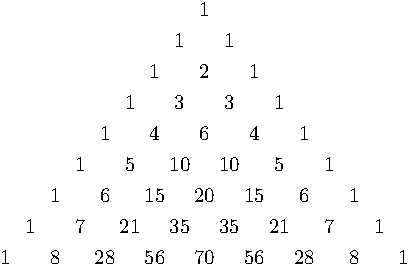
\includegraphics{image/tart-triangolo.pdf}
\end{center}

Ogni nuovo livello è costruito sul precedente sommando i due interi che
sovrastano un dato elemento in modo che il primo e l'ultimo numero siano sempre
1. La proprietà più nota del triangolo è che il livello \( n \) è formato dai
coefficienti binomiali \( (a + b)^n \).

Procediamo con il codice. Chiudete la guida e cercate una vostra implementazione
in \LuaTeX{} stampando i numeri dei livelli fino all'ottavo su una stessa linea
separandoli con uno spazio. Confrontate poi la soluzione fornita nel prossimo
listato.

Al solito stiamo procedendo per gradi. Otteniamo prima il codice che produce i
numeri del triangolo e poi il codice che costruisce la lista dei nodi da
inserire in una scatola che lo compone sulla pagina.

Ecco la mia versione, che utilizza una sola tabella che cresce livello dopo
livello:
\VerbatimInput{app-tartaglia/01.tex}


\section{Nodi}

I numeri del triangolo vanno posizionati in punti ben precisi. Otterremo
la disposizione geometrica regolando le distanze tra i gruppi di cifre in modo
che il centro del testo che rappresenta un numero sia sull'asse verticale
opportuno per il livello, e disponendo una scatola sull'altra per l'insieme dei
livelli. I passi che svolgeremo in plain \LuaTeX{} sono i seguenti:
\begin{compactenumerate}
\item comporre una cifra,
\item comporre un numero in una lista,
\item comporre più numeri in linea congiungendo le liste con un nodo spazio,
\item assemblare una scatola sull'altra.
\end{compactenumerate}


\subsection{Un numero}

Per costruire un nodo di tipo glifo, un singolo elemento nella collezione
di un font, si utilizza la funzione \fn{node.new}. Poi è obbligatorio
valorizzare almeno il codice del carattere per il campo \code{char} e il numero
del font per il campo \code{font}.

Ottenuto l'oggetto nodo possiamo comporlo sulla pagina con la funzione
\fn{node.write}. Per esempio se volessimo stampare un 8:
\VerbatimInput{app-tartaglia/02.tex}

La macro \cs{leavevmode} è importante perché è vietato inserire un oggetto glifo
in modo verticale, ed è questa la modalità in cui si trova \TeX{} all'inizio.


\subsection{Dal numero alla lista}

Dal numero, con l'operatore modulo a 10 è possibile ricavare in un ciclo le
cifre componenti la rappresentazione decimale a partire da quella meno
significativa. Con la singola cifra si crea il glifo e lo si concatena in una
lista tramite la funzione \fn{node.insert\_before} che funziona anche per
aggiungere un elemento in testa.

Curando il caso particolare dello zero, questo è quello che fa la funzione
\fn{digit} nel seguente sorgente compilabile:
\VerbatimInput{app-tartaglia/03.tex}

Il metodo \fn{node.write} accetta un nodo e non una lista. Ma se il nodo
argomento ha un riferimento a un nodo nel campo \code{next}, verrà composta
tutta la catena. Questi riferimenti sono stati inseriti per noi da
\fn{node.insert\_before}.

Dunque la lista costruita è la sequenza di glifi delle cifre del numero 12090.
Dobbiamo ricordarci che il testo composto che ne risulta è tipografia minimale,
perché la lista non è stata modificata per inserire legature, kerning, o punti
di cesura a fin di riga. Con i nodi siamo noi gli artigiani digitali.


\subsection{Numeri e spazi}

Un nodo \emph{glue} distanzia il nodo precedente da quello successivo, in
orizzontale. Può essere elastico in estensione o riduzione, oppure rigido.
Per il nostro scopo dovremo calcolare la distanza rigida tra i nodi in modo
tale che i centri dei due numeri successivi a un livello del triangolo distino
sempre lo stesso valore.

Occorre quindi misurare la larghezza del numero composto. La cosa più semplice è
inserire la lista dei nodi glifo in una scatola orizzontale per poi misurarla
con la funzione \fn{node.dimensions} che ne restituisce larghezza, altezza sulla
lina base e profondità dalla linea base.

La dimensione tra due scatole dovrà essere la differenza tra la distanza assiale
con la semisomma delle larghezze delle scatole adiacenti.

Il passo successivo è quindi aggiungere la funzione \fn{pack\_level} per
costruire la scatola orizzontale contentente la lista di un livello intero del
triangolo di Tartaglia a partire dalla tabella di interi.

Una scatola orizzontale di una lista si costruisce passando il nodo capolista
alla funzione \fn{node.hpack}. nel codice ho modificato la funzione \fn{digits}
affinché restituisca due paramentri: il nodo della scatola orizzontale che
contiene la lista dei nodi glifi e la larghezza della scatola stessa.

Il sorgente compilabile diventa questo:
\VerbatimInput{app-tartaglia/04.tex}

Se esageriamo con la grandezza dei numeri allora si sovrapporrano. Questo
succede se la lunghezza elastica è negativa poiché la distanza assiale di 24pt
(vedi la variabile locale \key{a}) è troppo piccola. A questo livello del
codice, l'utente deve controllare che non ci siano sovrapposizioni specie
all'ultima riga del triangolo dove si trovano i numeri più grandi.


\subsection{Sovrapposizione scatole}

Il passo finale è quello di sovrapporre le scatole orizzontali a formare il
triangolo. Basterà impacchettare le scatole in una scatola verticale con la
funzione \fn{node.vpack} dopo aver costruito la lista di scatole e spazi
verticali.

Dobbiamo prima modificare la funzione \fn{pack\_level} perché restituisca una
scatola orizzontale per il materiale di un intero livello. Fino a ora la lista
poteva anche essere una sequenza di scatole e nodi glue perché la immettevamo in
modo orizzontale. Adesso invece immettiamo le righe del triangolo in ambiente
verticale impacchettando la lista delle righe separate con un nodo di lunghezza
con la funzione \fn{node.vpack}.

Queste sono le nuove funzioni: \fn{next\_level} calcola la riga del triangolo
rispetto a quella precedente, e \fn{tartaglia} genera il triangolo fino al
livello specificato in una scatola verticale:
\lines
-- filename: app-tartaglia/05.tex
local function next_level(t, row)
    t[row+1] = 1
    for e = row, 2, -1 do
        t[e] = t[e] + t[e-1]
    end
end
local function tartaglia(level)
    assert(type(level)=="number")
    local il = tex.sp "8.5pt"
    local head, last
    local t = {}
    for l = 0, level do
        next_level(t, l)
        local hbox = pack_level(t)
        if head then
            local g = node.new("glue")
            g.width = il
            head, last = node.insert_after(head, last, g)
            head, last = node.insert_after(head, last, hbox)
        else
            head, last = node.insert_after(head, last, hbox)
        end
    end
    local vbox = node.vpack(head)
    return vbox
end
\endlines
\sourcecode{from_lines()}

Il risultato è questo:
\begin{center}
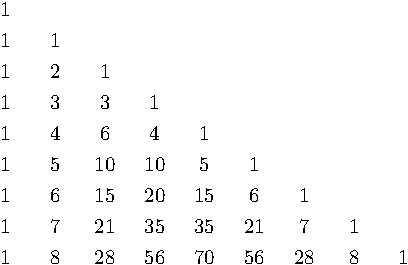
\includegraphics{image/tart-left}
\end{center}


\subsection{Opzione allineamento}

Per allineare al centro o a destra le linee possiamo introdurre dei nodi
lunghezza nella scatola orizzontale della singola riga. Conviene inserire questi
nodi con la funzione \fn{pack\_level} perché se lo facessimo all'esterno dovremo
poi reimpacchettare la lista in un'ulteriore scatola orizzontale per poterle poi
sovrapporre in ambiente verticale.

A questo scopo aggiungeremo il parametro \code{align}. Per dimostrare quanto si
riveli utile la dinamicità del linguaggio Lua, considereremo tre diversi
possibili gruppi di valori di tipo diverso per il parametro:
\begin{compactitemize}
\item \code{align} vale \key{nil}, per esempio perché nella chiamata di funzione
principale il valore non è stato assegnato: l'allineamento assume il valore di
default di triangolo centrato;
\item \code{align} è una stringa, allora potrà valere \code{"left"},
\code{"center"} o \code{"right"};
\item \code{align} è un numero come frazione di spazio che deve rimanere a
sinistra del primo elemento in alto. Quindi 0 è la stessa cosa dell'allineamento
\code{"left"}, \( 1/2 \) di \code{"center"} e 1 di \code{"right"}. Sono
possibili valori negativi o maggiori di 1.
\end{compactitemize}

Il trucco per implementare facilmente l'aggiunta delle lunghezze di allineamento
davanti e in coda alla lista degli elementi di un livello del triangolo è quello
di conoscere quanto vale lo spazio \( w \) da distribuire opportunamente.

Al livello \( r \), se \( a \) è la distanza assiale tra numeri adiacenti e \(
r_\mathrm{tot} \) è il numero totale dei livelli, allora \( w \) vale:
\[
w = k_\mathrm{left} + k_\mathrm{right} = a\left(r - r_\mathrm{tot}\right)
\]

L'esattezza matematica dell'espressione è dovuta al fatto che il numero in testa
e in coda per ogni riga del triangolo è sempre 1.

Il listato completo della funzione \fn{pack\_level} è il seguente:
\lines
-- filename: app-tartaglia/06.tex
local function pack_level(t, diff_level, k_left, k_right)
    local a = tex.sp "24pt"
    local w1
    local head, last
    if diff_level == 0 then
        k_left, k_right = nil, nil
    end
    if k_left then
        head = node.new("glue")
        head.width = a*diff_level*k_left
        last = head
    end
    for _, n in ipairs(t) do
        local hbox, w2 = pack_digits(n)
        if w1 then
            local g = node.new("glue")
            g.width = a - (w1+w2)/2
            w1 = w2
            head, last = node.insert_after(head, last, g)
            head, last = node.insert_after(head, last, hbox)
        else
            w1 = w2
            head, last = node.insert_after(head, last, hbox)
        end
    end
    if k_right then
        local g = node.new("glue")
        g.width = a*diff_level*k_right
        head, last = node.insert_after(head, last, g)
    end
    return node.hpack(head)
end
\endlines
\sourcecode{from_lines()}

La funzione tiene conto delle situazioni in cui non è necessario inserire il
distanziamento di allineamento su un lato, cioè quando la lunghezza vale zero
oppure quando la linea da impacchettare è l'ultima, riga che non ha mai
necessità di essere traslata.

Tuttavia, non viene fatto affidamento sulla \emph{direzione di composizione} per
allineare a destra o a sinistra e viene inserito sempre lo spazio. Se
l'allineamento fosse a sinistra le scatole sarebbero allineate a sinistra dal
compositore che dispone gli oggetti in modo orizzontale da sinistra a destra. Ma
se la direzione fosse impostata al contrario l'effetto sarebbe l'opposto.

Per questo nel codice viene inserita la lunghezza a destra nonostante
l'allineamento a sinistra. I parametri \( k_\mathrm{left} \) e \(
k_\mathrm{right} \) sono definiti dalla funzione principale \fn{tartaglia} a
seconda del parametro \code{align}. Il listato è il seguente:
\lines
-- filename: app-tartaglia/06.tex
local function tartaglia(level, align)
    assert(type(level)=="number")
    local k_left, k_right; if align then
        if type(align) == "string" then
            if align == "center" then
                k_left, k_right = 0.5, 0.5
            elseif align == "right" then
                k_right = 1
            elseif align == "left" then
                k_left = 1
            end
        elseif type(align) == "number" then
            if align == 0 then
                k_right = 1
            elseif align == 1 then
                k_left = 1
            else
                k_left, k_right = align, 1 - align
            end
        else
            error("Unexpected alignment value")
        end
    else
        k_left, k_right = 0.5, 0.5
    end
    local il = tex.sp "8.5pt"
    local head, last
    local t = {}
    for l = 0, level do
        next_level(t, l)
        local hbox = pack_level(t, level - l, k_left, k_right)
        if head then
            local g = node.new("glue")
            g.width = il
            head, last = node.insert_after(head, last, g)
            head, last = node.insert_after(head, last, hbox)
        else
            head, last = node.insert_after(head, last, hbox)
        end
    end
    local vbox = node.vpack(head)
    return vbox
end
\endlines
\sourcecode{from_lines()}

Domanda: se avessimo avuto numeri diversi da 1 come primo e ultimo elemento, se
ritenuto necessario, quali modifiche occorrebbe considerare nel codice?


\subsection{Verifica grafica degli allineamenti con TiKZ}

Per controllare visivamente gli allineamenti verticali nel triangolo di
Tartaglia è possibile sovrapporre linee verticali sottili di passo \( a \) al
disegno. Realizzare questo disegno è in realtà molto semplice poiché una volto
costruito il nodo del contenitore, la scatola può essere assegnata direttamente
a uno dei registri tramite indicizzazione della tabella \code{tex.box}:
\begin{Verbatim}
% !TeX program = LuaTeX
\newbox\tartbox % nuovo registro
\directlua{
    ... definizioni come prima
    tex.box.tartbox = tartaglia(8)
}
\box\tartbox
\bye
\end{Verbatim}

La macro \cs{box} è una primitiva di \TeX{}. Quello che fa è comporre sulla
pagina il contenuto del box indicato dalla control sequence che lo segue e poi
svuotarlo.

A questo punto è facile separare la costruzione del triangolo dal suo impiego, e
un esempio è proprio far espandere la scatola in una macro \cs{node} del
pacchetto grafico TiKZ:
\begin{Verbatim}
% !TeX program = LuaTeX
% filename: app-tartaglia/07.tex
\input tikz.tex
\newbox\tartbox
% ...
\directlua{
    ... definizioni come prima
    tex.box.tartbox = tartaglia(8)
}
\tikzpicture
\foreach \x in {-96,-72,...,96} {
\draw[blue] (\x pt,68pt) -- (\x pt,-68pt);
}
\foreach \x in {-84,-60,...,84} {
\draw[red] (\x pt,68pt) -- (\x pt,-68pt);
}
\node at (0, 0) {\box\tartbox};
\endtikzpicture
\bye
\end{Verbatim}

Le rette rosse e quelle ble distano 24pt una dall'altra. Sono posizionate a
partire dall'ascissa zero poiché TiKZ inserirà la scatola usando il suo punto
centrale nell'origine del sistema di riferimento.

Le linee rosse corrispondono alle posizioni dei numeri sui livelli dispari,
e quelle blu a quelle dei livelli pari. Il risultato è:
\begin{center}
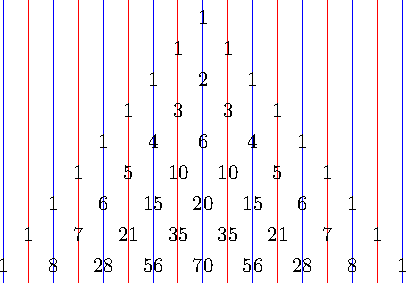
\includegraphics{image/tart-tikz.pdf}
\end{center}


\subsection{Regolazione automatica della distanza}

Sappiamo che la distanza \( a \) tra i centri di due numeri consecutivi su una
linea del triangolo è fissa. Se non fosse abbastanza grande i due numeri si
sovrapporrebbero e a quel punto l'utente dovrebbe reimpostarne il valore nel
sorgente e ricompilare.

Possiamo invece rendere l'operazione automatica e in diversi modi. Per esempio,
potremo intendere che il triangolo venga costruito in base a una distanza minima
tra un numero e l'altro, oppure impostando la distanza \( a \) come fissa per
incrementarla in caso di sovrapposizioni.

Una prima soluzione è costruire la scatola con il triangolo solo alla fine,
salvare cioè le scatole orizzontali dei numeri in una tabella e nel frattempo
calcolarne il valore minimo di \( a \); costruire poi la scatola contenitore del
triangolo distanziando opportunamente i nodi.

Una seconda strada è quella di impacchettare il triangolo come fatto fino a ora
negli esempi, per poi eventualmente scorrere la lista dei nodi per incrementare
la distanza tra i centri. Questa seconda strategia è quella che seguirò per
mostrare come una lista di nodi già costruita possa essere utilmente
modificata.


\subsection{Visitare la lista dei nodi}


\subsection{Modificare la distanza}

Useremo la funzione \fn{pack\_level} per creare la lista di un livello del
triangolo di Tartaglia già scritta in precedenza, e una nuova funzione
\fn{add\_distance} per modificare la distanza tra i centri.

Alcune informazioni utili tratte dal manuale di \LuaTeX{} che è bene richiamare:
la lista contenuta in un nodo scatola orizzontale o verticale inizia con il nodo
contenuto nel campo \code{head}. Nella lista il nodo successivo può essere
ricavato leggendo il campo \code{next} del nodo attuale. Il campo numerico
\code{id} indica il tipo di nodo, per esempio 12 individua un nodo \code{glue} e
0 un nodo \code{hbox}.

Aggiungere una distanza fissa è molto semplice. Sappiamo che il nodo \code{hbox}
è l'alternanza tra scatole orizzontali e nodi \code{glue}, perciò se \code{hbox}
è il mnome di variabile che contiene la scatola, il riferimento
\code{hbox.head.next} punta al primo nodo distanza. In un ciclo \key{while}
scorrere i soli nodi \code{glue} significa saltare un nodo e quindi preparare il
prossimo riferimento con il campo \code{glue.next.next}:
\lines
-- filename app-tartaglia/08.tex
local function add_distance(hbox, d)
    assert(hbox and hbox.id == 0)
    local glue = hbox.head.next
    while glue do
        assert(glue.id == 12)
        glue.width = glue.width + d
        glue = glue.next.next
    end
end
\endlines
\sourcecode{from_lines()}

Nel triangolo dobbiamo tener in conto tuttavia degli eventuali nodi di
spaziatura iniziale e finale per l'allineamento orizzontale del triangolo. In
questi spazi l'incremento della distanza è proporzionale alla differenza tra il
numero dei livelli totali con il numero di quello corrente. Dovremo adattare la
funzione \fn{add\_distance} per modificare le lunghezze non solo dei nodi
intermedi tra un numero e l'altro, ma anche per gli eventuali spazi di
allineamento citati, in questo modo:
\lines
-- filename app-tartaglia/09.tex
local function add_distance(hbox, d, k_left, k_right, level, totlevel)
    assert(hbox and hbox.id == 0)
    local glue = hbox.head
    local tdist = d*(totlevel - level)
    if k_left then
        assert(glue.id == 12)
        glue.width = glue.width + tdist*k_left
        glue = glue.next
    end
    glue = glue.next
    for _= 1, level do
        assert(glue.id == 12)
        glue.width = glue.width + d
        glue = glue.next.next
    end
    if k_right then
        assert(glue.id == 12)
        glue.width = glue.width +  tdist*k_right
    end
end
\endlines
\sourcecode{from_lines()}

Non si utilizza il ciclo \code{while} ma un ciclo \code{for} che itera tante
volte quanti sono gli spazi nel livello, ovvero il numero del livello a
cominciare da 1 perché il livello 0 non ha spazi intermedi. In questo modo è più
semplice per il codice gestire il puntatore al nodo invece che passare da un
nodo al successivo.

La versione finale contenuta nel file \code{app-tartaglia/09.tex}, conta 160
linee di codice Lua in grado di generare il triangolo di Tartaglia con il numero
di livelli richiesti, diverse opzioni di allineamento orizzontale, e con la
capacità di mantenere la distanza assiale tra i numeri di 24pt più l'eventuale
distanza perché ci siano almeno 3pt tra due numeri consecutivi.



Domanda: se e come cambiereste il codice per considerare la simmetria dei numeri
sulla riga di uno stesso livello del triangolo di Tartaglia?


\section{Riepilogo}

La tecnologia dei nodi consente di comporre oggetti tipografici di complessità
arbitraria. Seguendo vari passi di sviluppo, in questo capitolo abbiamo
costruito con essa il triangolo di Tartaglia, un esempio applicativo
interessante proprio per poter implementare nuove funzionalità come quella di
rendere variabile l'allineamento o lasciare che sia il codice ad aggiustare la
distanza tra i numeri se necessario.

Rimane da esplorare la gestione in Lua delle opzioni e dei parametri perché
l'utente possa modificare l'aspetto del triangolo. Considero questo tema
separato da quello dei nodi di \LuaTeX{}. Per questo motivo l'esercitazione
può dirsi conclusa.


% end of file


%

\chapter{Disegno del cerchio}
\label{iichCerchio}

In questo capitolo esploreremo un'altro tipo di nodo: il \emph{pdfliteral}.
Con esso possono essere inserite nel file PDF figure vettoriali definite
attraverso istruzioni grafiche. Per questi nodi il compositore non fa altro che
inserirli direttamente e senza alcun controllo nel file di uscita perché siano
interpretati unicamente dal programma di visualizzazione e stampa PDF.

Dovremo quindi prestare attenzione alla correttezza delle istruzioni che
definiamo seguendo la sintassi prevista dal formato PDF e contenuta nel PDF
reference distribuito da Adobe. Un errore potrebbe invalidare l'intero
documento.

Se si è utenti del sistema \TeX{} ci sarà certamente capitato di dover
realizzare diagrammi o figure, perciò abbiamo già utilizzato le istruzioni
pdfliteral ma non direttamente. I pacchetti grafici come \pack{picture2e} o
\pack{TikZ} infatti, offrono un'interfaccia di alto livello più compatta e
sicura alle primitive grafiche PDF.

Per conoscere questo tipo di tecnologia, implementeremo in Lua il disegno di
cerchi.


\section{Le curve di Bezier}


\section{Cerchio a otto curve}


\section{SVG}





% end of file


%

\chapter{Dati esterni}
\label{iichDati}

Il tema molto vasto di questo capitolo è la tecnologia che ci permette di
includere nei documenti dati esterni. Può capitare di voler comporre un buon
numero di documenti che condividono un insieme di dati, oppure di comporre un
documento che riporti tabelle con dati sperimentali residenti in file esterni.

Nel primo caso, vorremmo evitare di digitare sempre gli stessi dati in ciascun
documento con il rischio di sbagliare, mentre nel secondo cercheremo una
procedura che carichi in automatico i dati all'interno del documento
presentandoli con aspetto professionale.

Oppure ancora, potremo trovarci in ambito aziendale dove i dati che dovremo
includere nei documenti sono responsabilità di unità operative diverse dalla
nostra. Cercheremo un modo per condividere le informazioni in modo efficiente e
sicuro.

Gli scenari sono quindi molto vari e di conseguenza le tecnologie utili possono
essere le più diverse, per esempio nel fornire o meno la lettura sincrona dei
dati da un database. Comunque sia presenterò degli esempi concreti solamente per
contesti di gestione dati in cui è il motore di composizione a compiere le
elaborazioni affinché i dati siano disponibili all'interno del sorgente. A
questo ambito daremo il nome di \emph{progetti documentali}.

Per esempio, non è un progetto di documento quello in cui il programma elabora i
dati e crea il relativo file di testo che rappresenta il sorgente \TeX{}.
Infatti, così facendo non solo sarebbe possibile compilare il sorgente con i
compositori tradizionali come PDF\LaTeX{} o Xe\LaTeX{}, e quindi non saremo in
tema, ma non lavoreremo scrivendo il sorgente in modo diretto, ovvero nel
contesto ideale per comporre documenti complessi che contengono variazioni uno
rispetto all'altro sia nel contenuto sia nella struttura.


\section{Lua table}

Il modo più semplice per includere dati esterni è quello che non richiede la
scrittura di alcun modulo per caricare i dati. In altre parole, i dati devono
essere scritti secondo un formato nativo del linguaggio, nel nostro caso Lua.

Questo formato nativo per Lua non può che essere il costruttore di tabelle, che
abbiamo incontrato al capitolo~\ref{iChTabella}. Applicheremo questa fantastica
tecnica per realizzare modi diversi di presentare gli stessi dati.








%\subsection{Lua type}


%\subsection{SQLite3 e i quadri economici}


%\subsection{Matematica simbolica}

% end of file


\appendix

%


Come tutti i linguaggi di scripting non occorre compilare il codice Lua. Basta
scrivere il programma in un file di testo --- preferibilmente assegnandogli
l'estensione \key{.lua} --- e lanciare il comando d'esecuzione in un terminale
\tcmd{\$ lua nomefile}.

Per scrivere il codice vi consiglio di utilizzare l'editor
\href{http://www.scintilla.org/SciTE.html}{SciTE} perché è già predisposto per
eseguire programmi Lua ed è programmabile in Lua. Tra l'altro l'output del
programma viene visualizzato nella \emph{output tab}. Il tasto funzione F5
esegue il programma visualizzato nella scheda attiva in quel momento e il tasto
F8 attiva/disattiva la finestra di output, che è in pratica un terminale
incorporato nell'editor.

Prepariamoci a scrivere il primo programma in Lua, ovviamente il fatidico
\href{http://en.wikipedia.org/wiki/%22Hello,_world!%22_program"}{Hello world!},
salvando il seguente codice in un file chiamato \key{primo.lua} ed eseguiamolo
direttamente in SciTE premendo il tasto funzione F5 o al terminale con il
comando \tcmd{\$ lua primo.lua}:
\lines
print("Hello world!")
\endlines
\sourcecode{from_lines():add_output()}

In ambiente Linux o Mac OS~X, come per tutti gli altri linguaggi di scripting,
possiamo inserire come prima riga del file a cui sono stati assegnati i permessi
di esecuzione, la
\href{http://en.wikipedia.org/wiki/Shebang_%28Unix%29}{Sha-Bang}. In questo modo
basterà semplicemente scriverne il nome nel terminale, e in questo caso è
conveniente omettere l'estensione. Ecco il programma con la Sha-Bang:
\lines
#!/usr/bin/env lua
print("Hello world!")
\endlines
\sourcecode{from_lines()}

Lua è in grado di passare al programma gli argomenti che l'utente digita nel
terminale separandoli da spazi, tramite la tabella array chiamata \key{arg} che
conterrà all'indice 0 il nome dello script, e ai successivi indici i vari
argomenti utente come tipo stringa. Questa proprietà assieme alla tecnica della
sha-bang, dà all'utente la possibilità di scrivere programmi in Lua come se
fossero comandi da terminale, almeno per gli ambienti di classe *nix.

\chapter{Preparazione di un interprete Lua}

Poiché l'interprete Lua non interferisce con \LuaTeX{} e occupa una quantità di
memoria davvero piccola, è consigliabile installarlo per poter usare il modo
interattivo REPL e per sperimentare più comodamente.

Per seguire queste chiaccherate andrà benissimo una versione di Lua uguale o
superiore alla 5.1. Tuttavia è preferibile installare la versione che
corrisponde a quella inclusa in \LuaTeX{}, che viene riportata anche nel suo
manuale.

L'interprete Lua è scritto in Ansi~C e per questo è disponibile praticamente
per tutte le piattaforme, eventualmente compilandone i sorgenti.

Per verificare l'installazione è possibile dare il seguente comando da
terminale per stampare la versione dell'interprete:
\begin{Verbatim}
    $ lua -v
    Lua 5.2.3  Copyright (C) 1994-2013 Lua.org, PUC-Rio
\end{Verbatim}



\subsection{Linux}

Per i sistemi Linux fate ricorso al package manager della vostra distribuzione,
per esempio per le distribuzioni Debian e derivate come Ubuntu, è sufficiente
dare il comando:
\begin{Verbatim}
    $ sudo apt-get install lua
\end{Verbatim}



\subsection{Windows}

Per Windows fate riferimento alla pagina
\href{http://luabinaries.sourceforge.net/index.html}{LuaBinaries}. In caso di
problemi potete scaricare un file autoinstallante dal progetto
\href{https://github.com/rjpcomputing/luaforwindows}{Lua for Windows} fermo
però alla versione 5.1.5 di Lua ma completo di alcune librerie utili.



\subsection{Mac OSX}

Per Mac OSX andate alla pagine \href{http://rudix.org/packages/lua.html}{Rudix}
e individuate il package adatto per la versione del vostro Mac.



\section{Come eseguire il codice}

Operativamente, ci sono molti modi per eseguire codice Lua. La modalità usuale
è installarne l'interprete e questo capitolo riporta le procedure per i tre
principali sistemi operativi.

Se si dispone di una recente distribuzione del sistema \TeX{}, per esempio
TeX~Live, uno \emph{script} in Lua può anche essere eseguito da \LuaTeX{}, per
esempio con il comando da terminale:
\begin{Verbatim}
$ luatex --luaonly nomefile
\end{Verbatim}

Nella parte~\ref{partLuaTeX} vedremo come sia possibile inserire il codice Lua
all'interno di un sorgente \texttt{.tex}. Per esempio, poiché sto componendo
questa guida in \LuaLaTeX{} --- che altro non è che \LuaTeX{} con il formato
\LaTeX{} precaricato --- scrivendo il codice:
\begin{Verbatim}
\directlua{tex.print(lua.version)}
\end{Verbatim}
posso dirvi che la versione di Lua inclusa è \directlua{tex.print(lua.version)}.


\subsection{Modalità interattiva}

Aprite un terminale, o console in Windows, e digitate semplicemente il comando
\texttt{lua}. Entreremo nella modalità interattiva dove potremo
digitare istruzioni una alla volta. Per uscire tornando al prompt, digitate la
funzione \texttt{os.exit()} seguita da un bel tasto invio.

In modalità interattiva possiamo comodamente controllare quale tipo ha un
valore, utilizzando la funzione \texttt{type()}. Essa restituisce una stringa
che corrisponde al nome del tipo di un'espressione, stringa che possiamo a sua
volta stampare con la funzione \texttt{print()} in console. Digitiamo
\footnote{Il doppio trattino inserisce un commento di riga.}:
\lines
a = 123
print(type(123))    --> stampa "number"
print(type(a))      --> stampa "number"
print(type("123"))  --> stampa "string"
\endlines
\sourcecode{from_lines()}


% end of file



\backmatter



\chapter{Note finali}

I miei ringraziamenti vanno a Claudio Beccari per aver scritto la classe
\class{guidatemaica.cls} con cui è stata composta la guida.

% end of file


% \input{section/9-end/02-colophone}

% bibliografia
\end{document}

